\documentclass[11pt]{article}
\usepackage[margin=1in]{geometry}
\usepackage{booktabs}
\usepackage{tabularx}
\usepackage{float}
\usepackage{xcolor}
\usepackage{siunitx}
\usepackage{graphicx}
\usepackage{caption}
\usepackage{hyperref}
\usepackage{enumitem}
\setlist{nosep}
\hypersetup{colorlinks=true,linkcolor=black,urlcolor=blue}

\newcommand{\pass}{\textcolor{green!50!black}{\textbf{PASS}}}
\newcommand{\fail}{\textcolor{red!70!black}{\textbf{FAIL}}}

\title{2.4\,GHz FMCW Radar --- Simulation Results}
\author{David Brown}
\date{October 2026}

\begin{document}
\maketitle

\noindent The horn antenna was simulated in Ansys HFSS (Student 2025 R2) and the baseband board in
NI Multisim 14.2 using library parts. Nothing has been built yet. Plots for every check are in
Section~\ref{sec:figs}.

\section{Horn antenna (HFSS)}

Pyramidal horn on WR-340, mouth $263.8 \times 193.1$\,mm, coax probe feed.
Band: 2400--2483.5\,MHz.

\begin{table}[H]
\centering
\small
\begin{tabularx}{\linewidth}{>{\raggedright\arraybackslash}X>{\raggedright\arraybackslash}p{3.3cm}>{\raggedright\arraybackslash}p{2.6cm}l}
\toprule
Check & Result & Requirement & \\
\midrule
Match (S11), worst in band, original probe (28 / 43.7\,mm) & $-5.2$\,dB & $\le -10$\,dB & \fail \\
Match (S11), worst in band, final probe (27 / 17.7\,mm) & $-24.3$\,dB & $\le -10$\,dB & \pass \\
Gain at 2.400 / 2.442 / 2.483\,GHz & 13.24 / 13.24 / 13.27\,dBi & 12.5--14\,dBi & \pass \\
Beamwidth, E / H plane & $34.4^\circ$ / $36.4^\circ$ & theory $33.4^\circ$ / $35.2^\circ$ & \pass \\
TX $\to$ RX leakage, horns 290\,mm apart & $-49.4$\,dB & $\le -35$\,dB & \pass \\
Match with probe off by $\pm1$\,mm & $-14.5$\,dB & $\le -10$\,dB & \pass \\
Mesh check (8.8k / 11.9k / 28.8k cells) & 0.14\,dB gain spread & $\le 0.2$\,dB & \pass \\
Copper walls vs.\ perfect conductor & $+0.01$\,dB gain & $\le 0.2$\,dB & \pass \\
\bottomrule
\end{tabularx}
\end{table}

\noindent\textbf{Change made:} probe moved from 28\,mm long, 43.7\,mm from the back wall, to
27\,mm long, 17.7\,mm from the back wall (picked from a 1\,mm sweep of 57 runs).

\section{Baseband board (Multisim)}

\begin{table}[H]
\centering
\small
\begin{tabularx}{\linewidth}{>{\raggedright\arraybackslash}p{2.3cm}>{\raggedright\arraybackslash}X>{\raggedright\arraybackslash}p{3.1cm}>{\raggedright\arraybackslash}p{3.1cm}l}
\toprule
Card & Check & Result & Requirement & \\
\midrule
1 Video amp & Outputs at half rail (DC) & 1.07\,mV off & $\le 150$\,mV & \pass \\
 & Gain at 159\,Hz / 1\,kHz / 15.9\,kHz & 48.7 / 54.5 / 50.9\,dB & 48.7 / 54.5 / 50.6\,dB & \pass \\
 & 0.5\,mV, 1\,kHz in & 0.266\,V out & 0.27\,V & \pass \\
 & First power-up gain, 10\,mV in & 106.8\,mV out & 107\,mV & \pass \\
 & Clipping & $\pm4.06$\,V & about $\pm4.2$\,V & \pass \\
 & Two-tone: 417 / 870\,Hz lines & 19.1 / 21.1\,mV & 19.0 / 21.2\,mV & \pass \\
2 Half-rail ref & Divider / buffered output & 5.70 / 5.58\,V & 5.70 / 5.58--5.72\,V & \pass \\
 & 150\,kHz ripple reaching vref & $-162$\,dB & $\le -100$\,dB & \pass \\
3 12\,V input & Protected / analog rail & 11.72 / 11.62\,V & 11.68 / 11.58\,V & \pass \\
 & Ripple on analog rail & 3.2\,mVpp & about 4\,mVpp & \pass \\
4 Reverse supply & $-12$\,V applied & $-11$\,mV gets through & $< 0.5$\,V & \pass \\
5 Sync divider & Sync pulse level & 275\,mV & 270--300\,mV & \pass \\
6 IF input & At 417\,Hz / 2.44\,GHz & $-6.6$ / $-57.7$\,dB & $-6.6$ / $-57.7$\,dB & \pass \\
7 Scaled radar & Beat tone at 5 / 10 / 15\,m & 435.0 / 870.7 / 1305.8\,Hz & 435.2 / 870.4 / 1305.6\,Hz & \pass \\
 & Beat tone with leakage on & 872.7\,Hz & stays at 870\,Hz & \pass \\
8 Full board (as built) & Outputs at half rail (DC) & 4.36\,V off & $\le 150$\,mV & \fail \\
8 Full board (fixed) & Outputs at half rail (DC) & 1.08\,mV off & $\le 150$\,mV & \pass \\
 & Gain vs.\ card 1 (C6 = 47\,\textmu F) & 6.4\,dB low & within 0.3\,dB & \fail \\
 & Gain vs.\ card 1 (C6 = 3.3\,mF) & 0.15\,dB & within 0.3\,dB & \pass \\
 & Two-tone 870\,Hz line & 21.0\,mV & 21.2\,mV & \pass \\
 & 150\,kHz ripple at output & 0.06\,\textmu V & $< 1$\,mV & \pass \\
 & Power-up from 6\,V & settles in 0.53\,s & $< 1$\,s & \pass \\
\bottomrule
\end{tabularx}
\end{table}

\noindent\textbf{Changes made on card 8:}
\begin{itemize}
  \item Wired U1A's $V-$ and U1B's $V+$ pins. They were left unconnected when the blocks were
        copied onto one sheet, which latched the amp at the rail.
  \item C6 raised from 47\,\textmu F to 3.3\,mF. The half-rail reference was moving with the
        signal and the first stage amplified it.
\end{itemize}

\noindent\textbf{Notes:}
\begin{itemize}
  \item Card 8's analog rail reads 11.49\,V because the TI op-amp model draws 5.7\,mA per amp
        (datasheet: 1.4\,mA typ.). Expected about 11.6\,V on the real board.
  \item The op-amp model can't run below about 4.4\,V supply, so power-up starts at 6\,V.
\end{itemize}

\section{Summary}

\begin{itemize}
  \item Horn: all checks pass after the probe move.
  \item Baseband: all cards pass. Card 8 passes after the wiring fix and the C6 change.
\end{itemize}

\clearpage
\section{Figures}\label{sec:figs}
\subsection*{Horn antenna (HFSS)}
\begin{figure}[H]\centering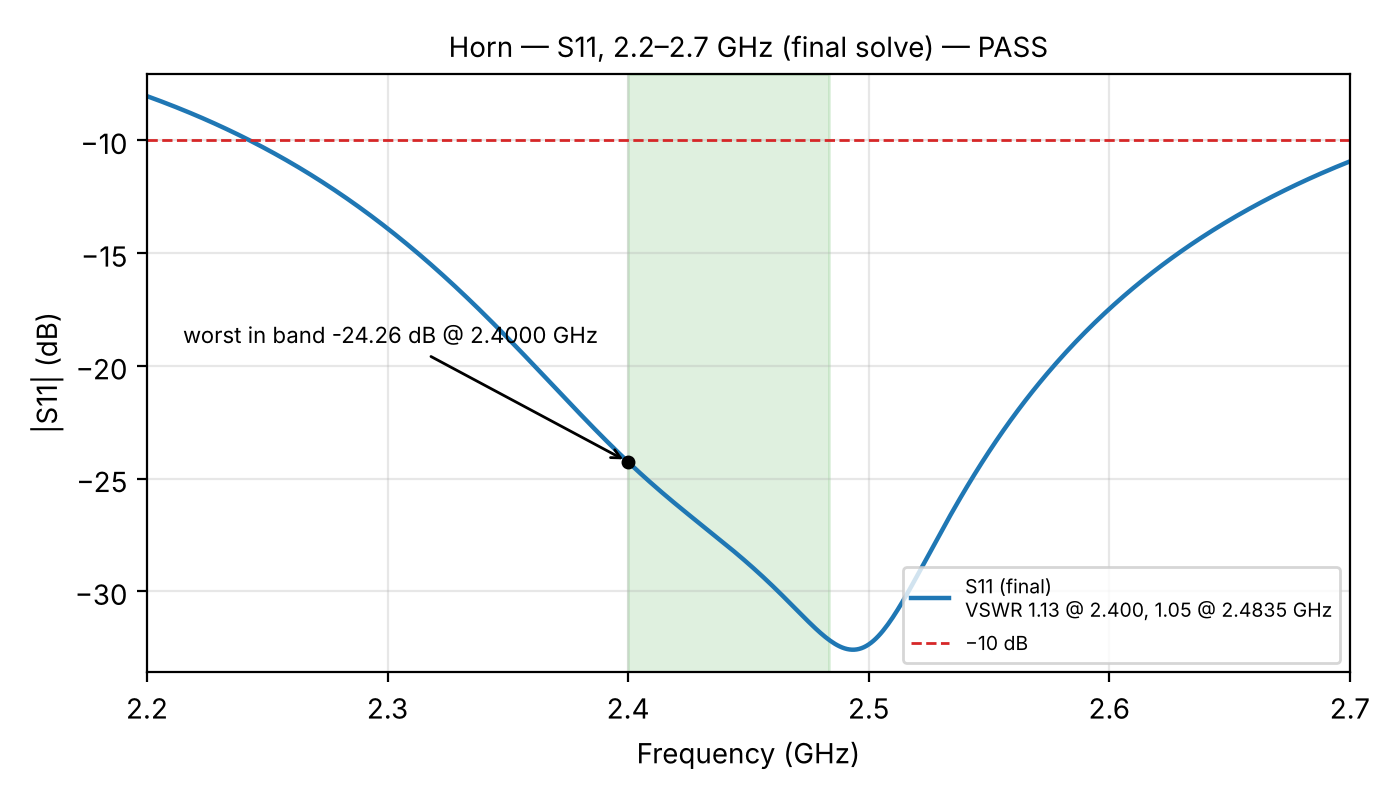
\includegraphics[width=0.85\linewidth,height=0.4\textheight,keepaspectratio]{figures/hfss/s11}\caption{Match (S11) across the band, final probe}\end{figure}
\begin{figure}[H]\centering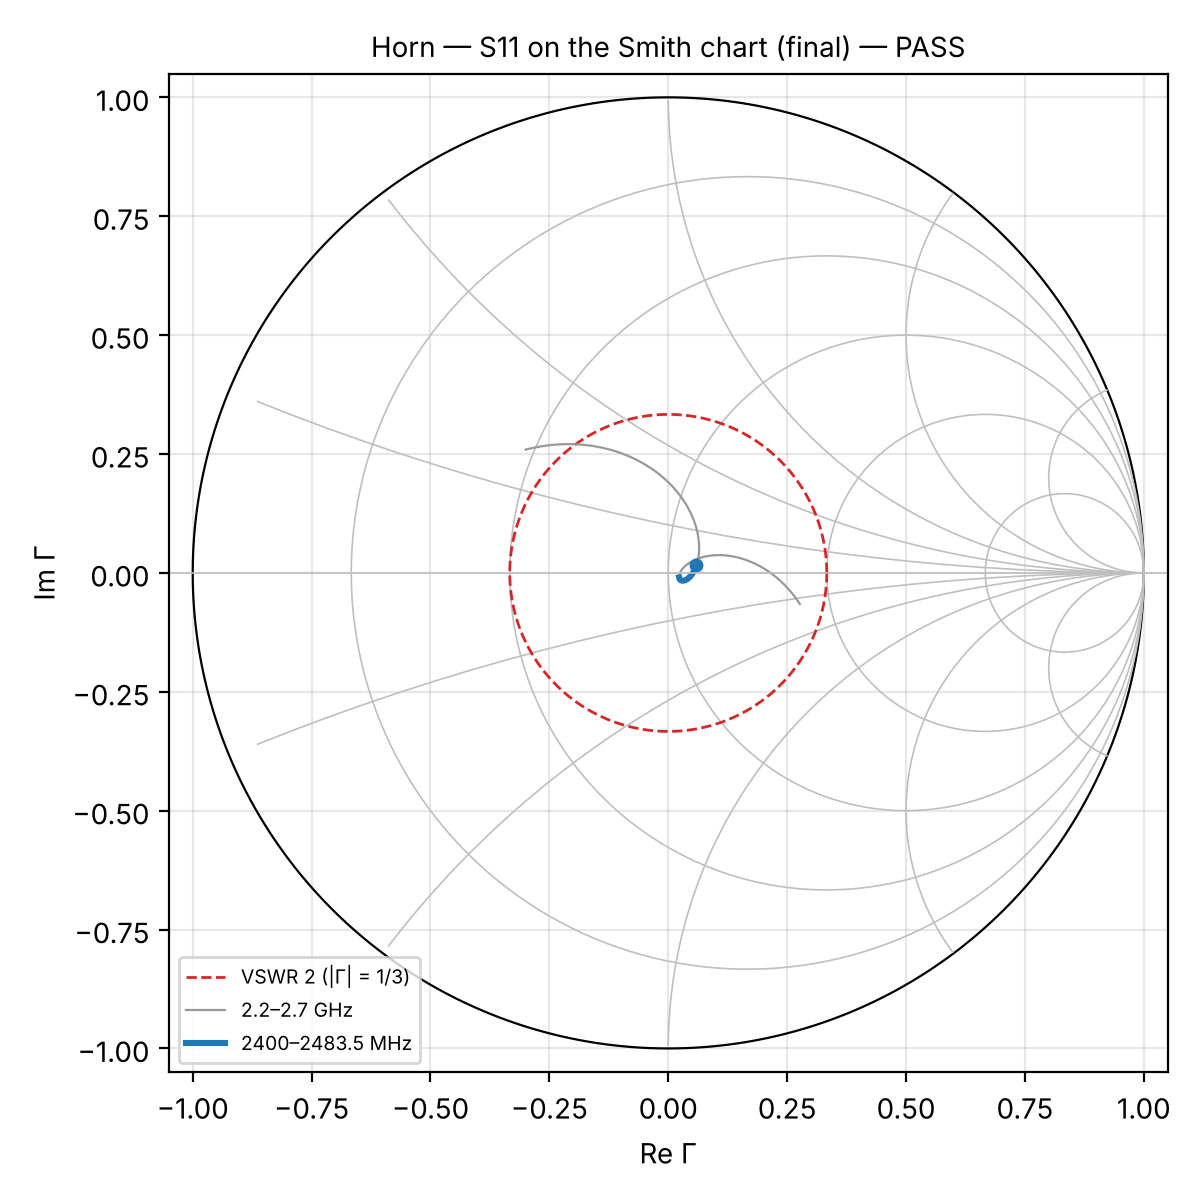
\includegraphics[width=0.85\linewidth,height=0.4\textheight,keepaspectratio]{figures/hfss/smith}\caption{Smith chart, final probe}\end{figure}
\begin{figure}[H]\centering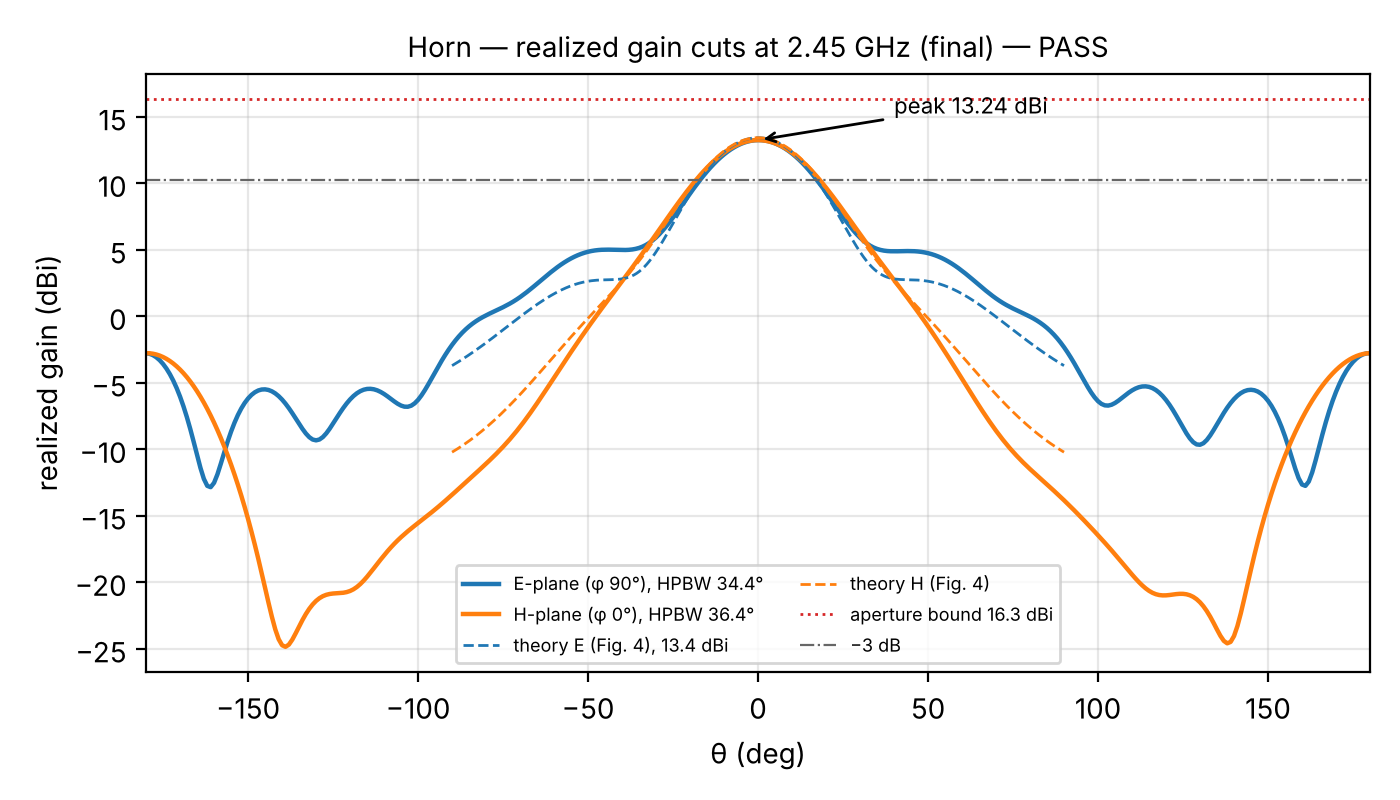
\includegraphics[width=0.85\linewidth,height=0.4\textheight,keepaspectratio]{figures/hfss/patterns}\caption{Gain patterns, E and H plane}\end{figure}
\begin{figure}[H]\centering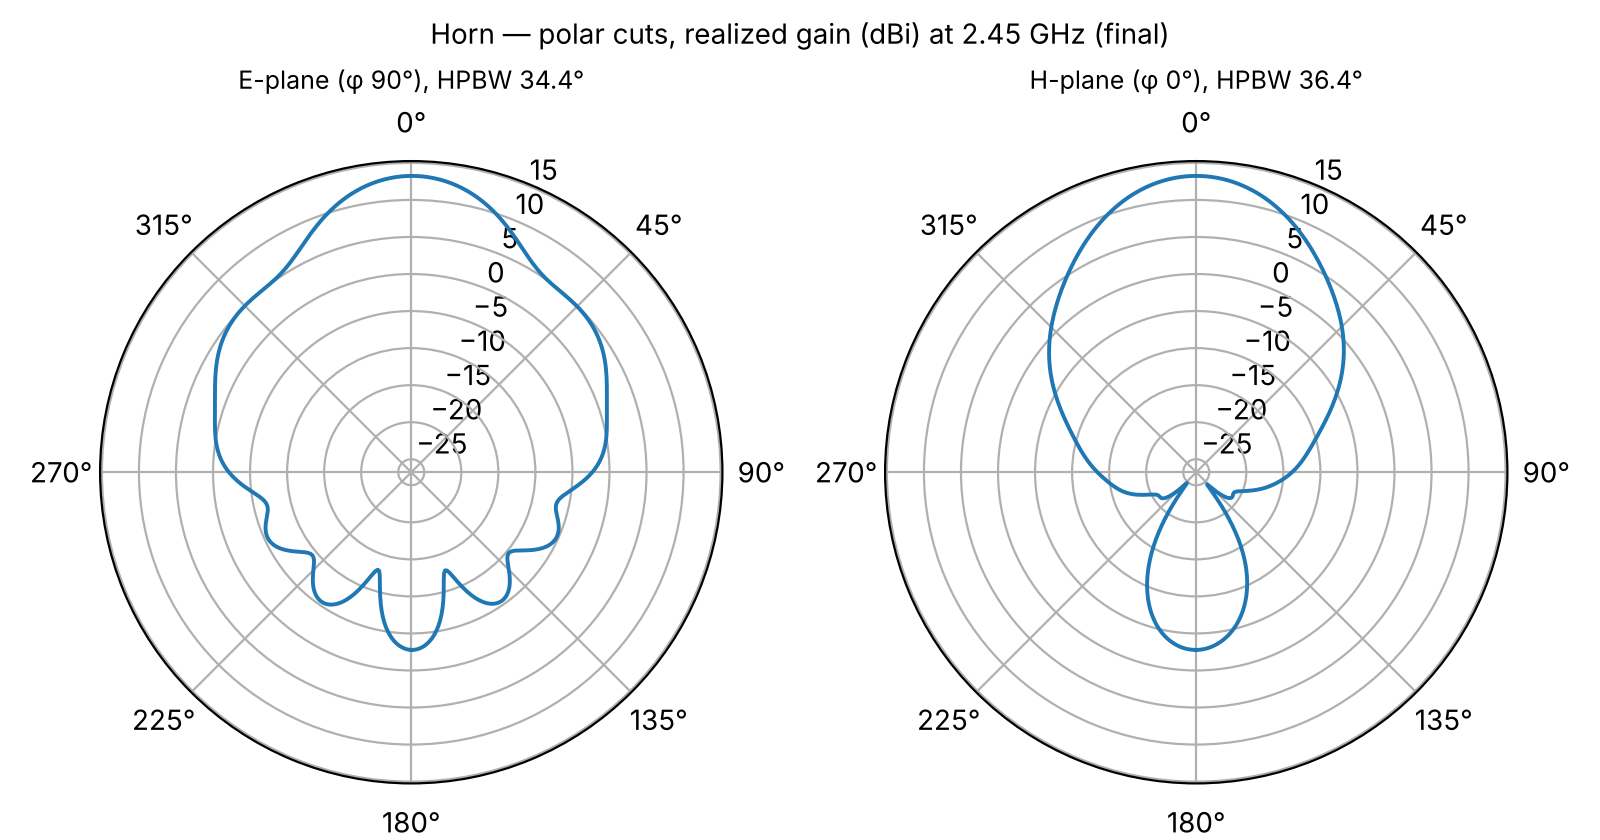
\includegraphics[width=0.85\linewidth,height=0.4\textheight,keepaspectratio]{figures/hfss/patterns_polar}\caption{Gain patterns, polar}\end{figure}
\begin{figure}[H]\centering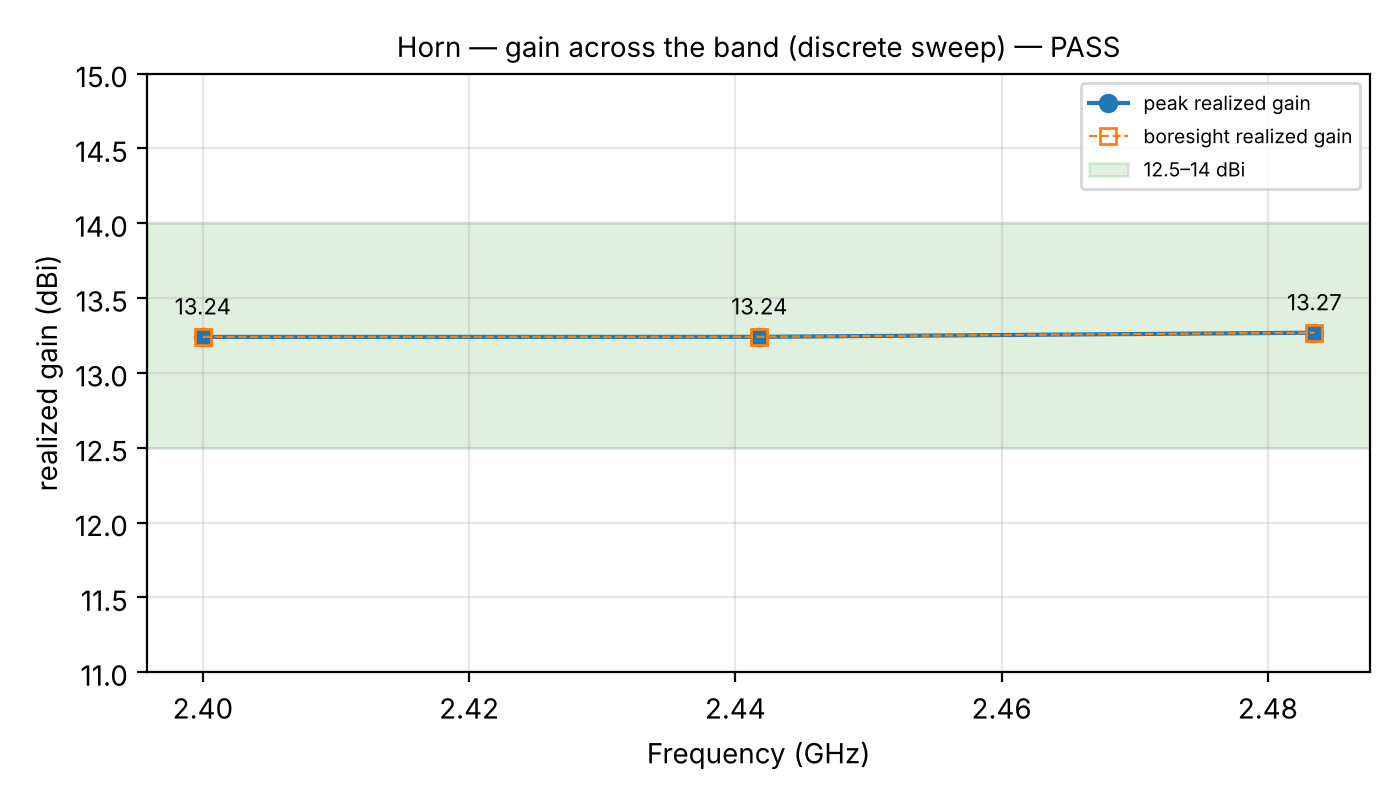
\includegraphics[width=0.85\linewidth,height=0.4\textheight,keepaspectratio]{figures/hfss/gain_vs_freq}\caption{Gain straight ahead across the band}\end{figure}
\begin{figure}[H]\centering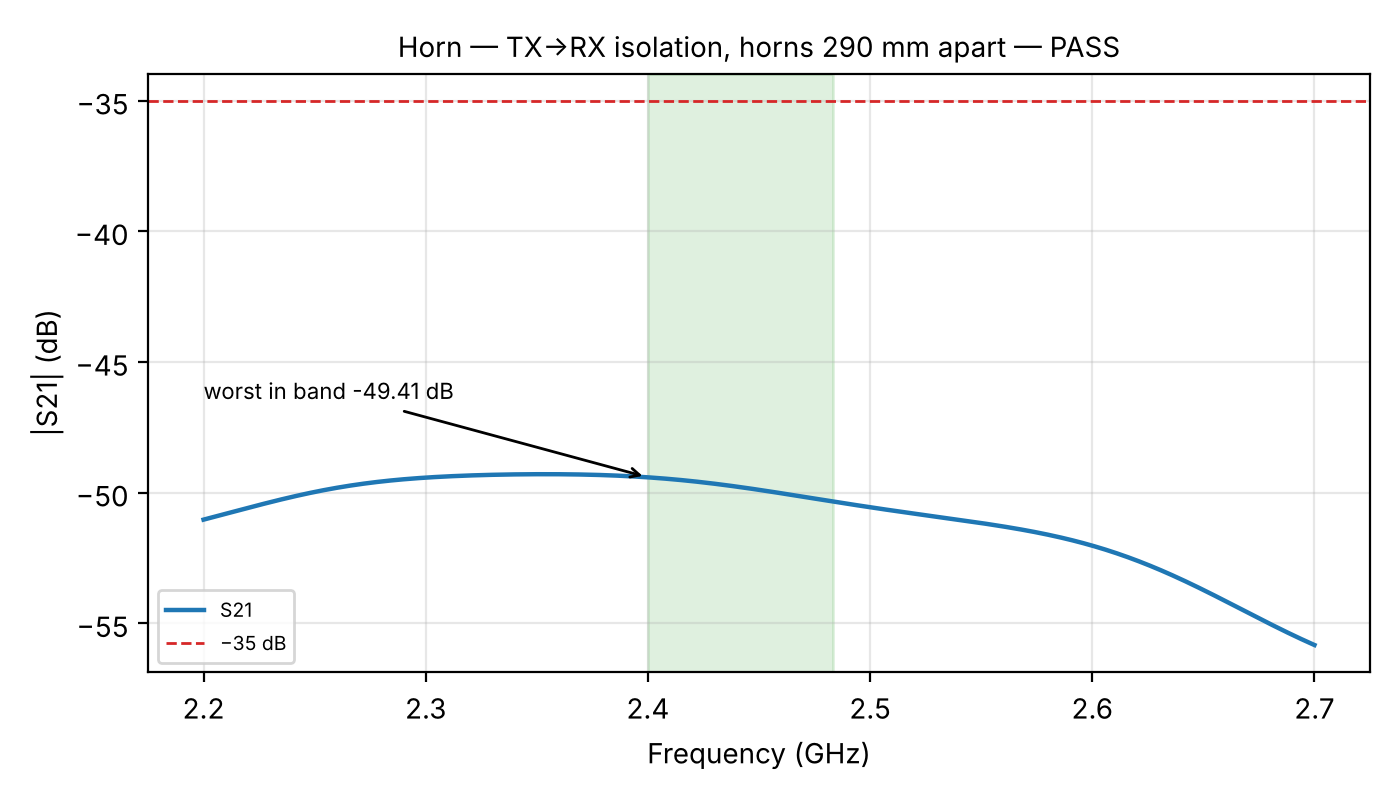
\includegraphics[width=0.85\linewidth,height=0.4\textheight,keepaspectratio]{figures/hfss/isolation}\caption{TX to RX leakage, horns 290 mm apart}\end{figure}
\begin{figure}[H]\centering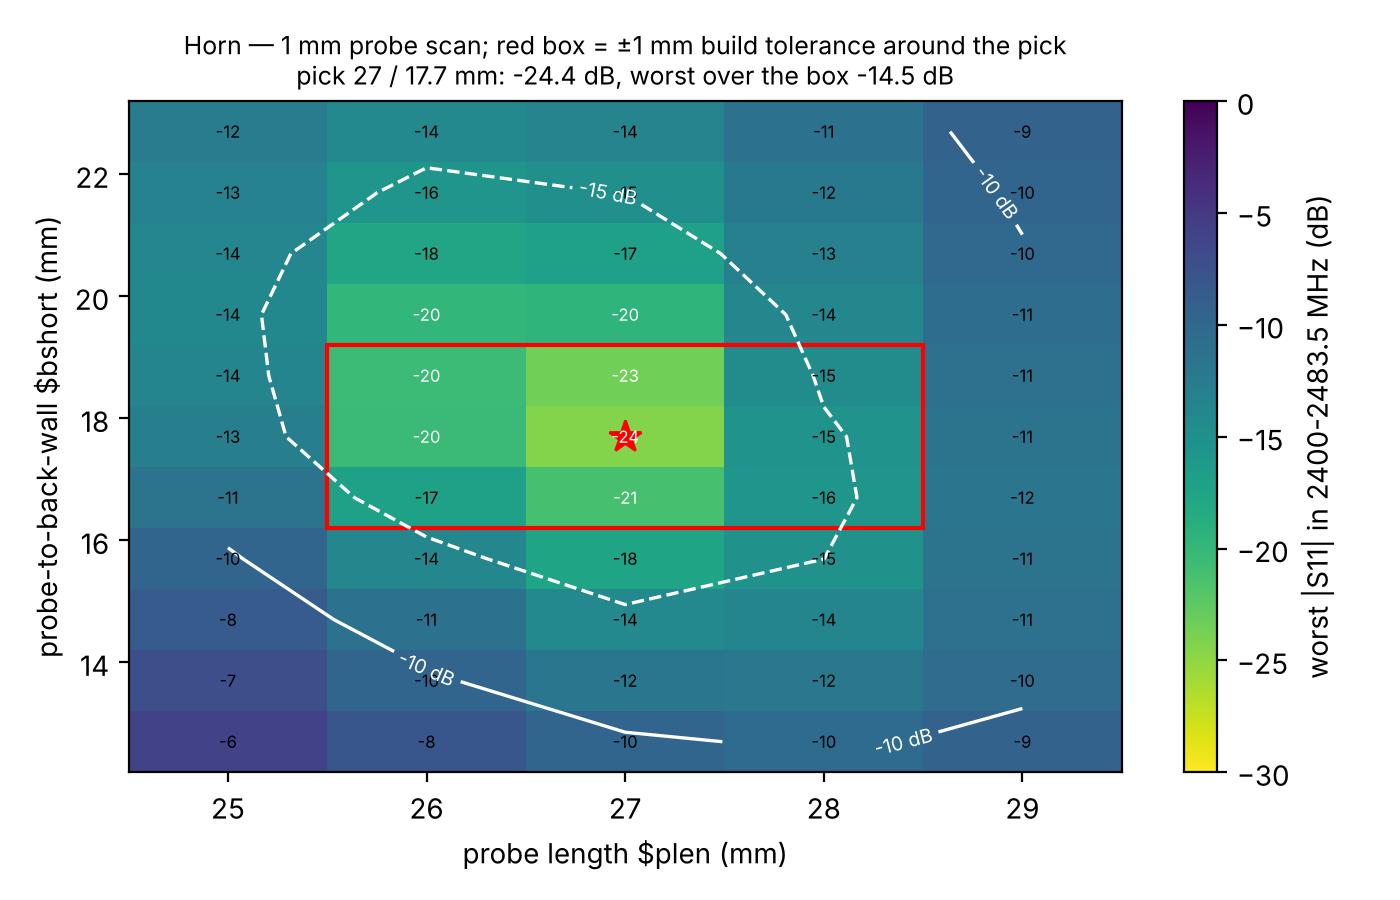
\includegraphics[width=0.85\linewidth,height=0.4\textheight,keepaspectratio]{figures/hfss/scan_heatmap}\caption{1 mm probe sweep: worst match in band}\end{figure}
\begin{figure}[H]\centering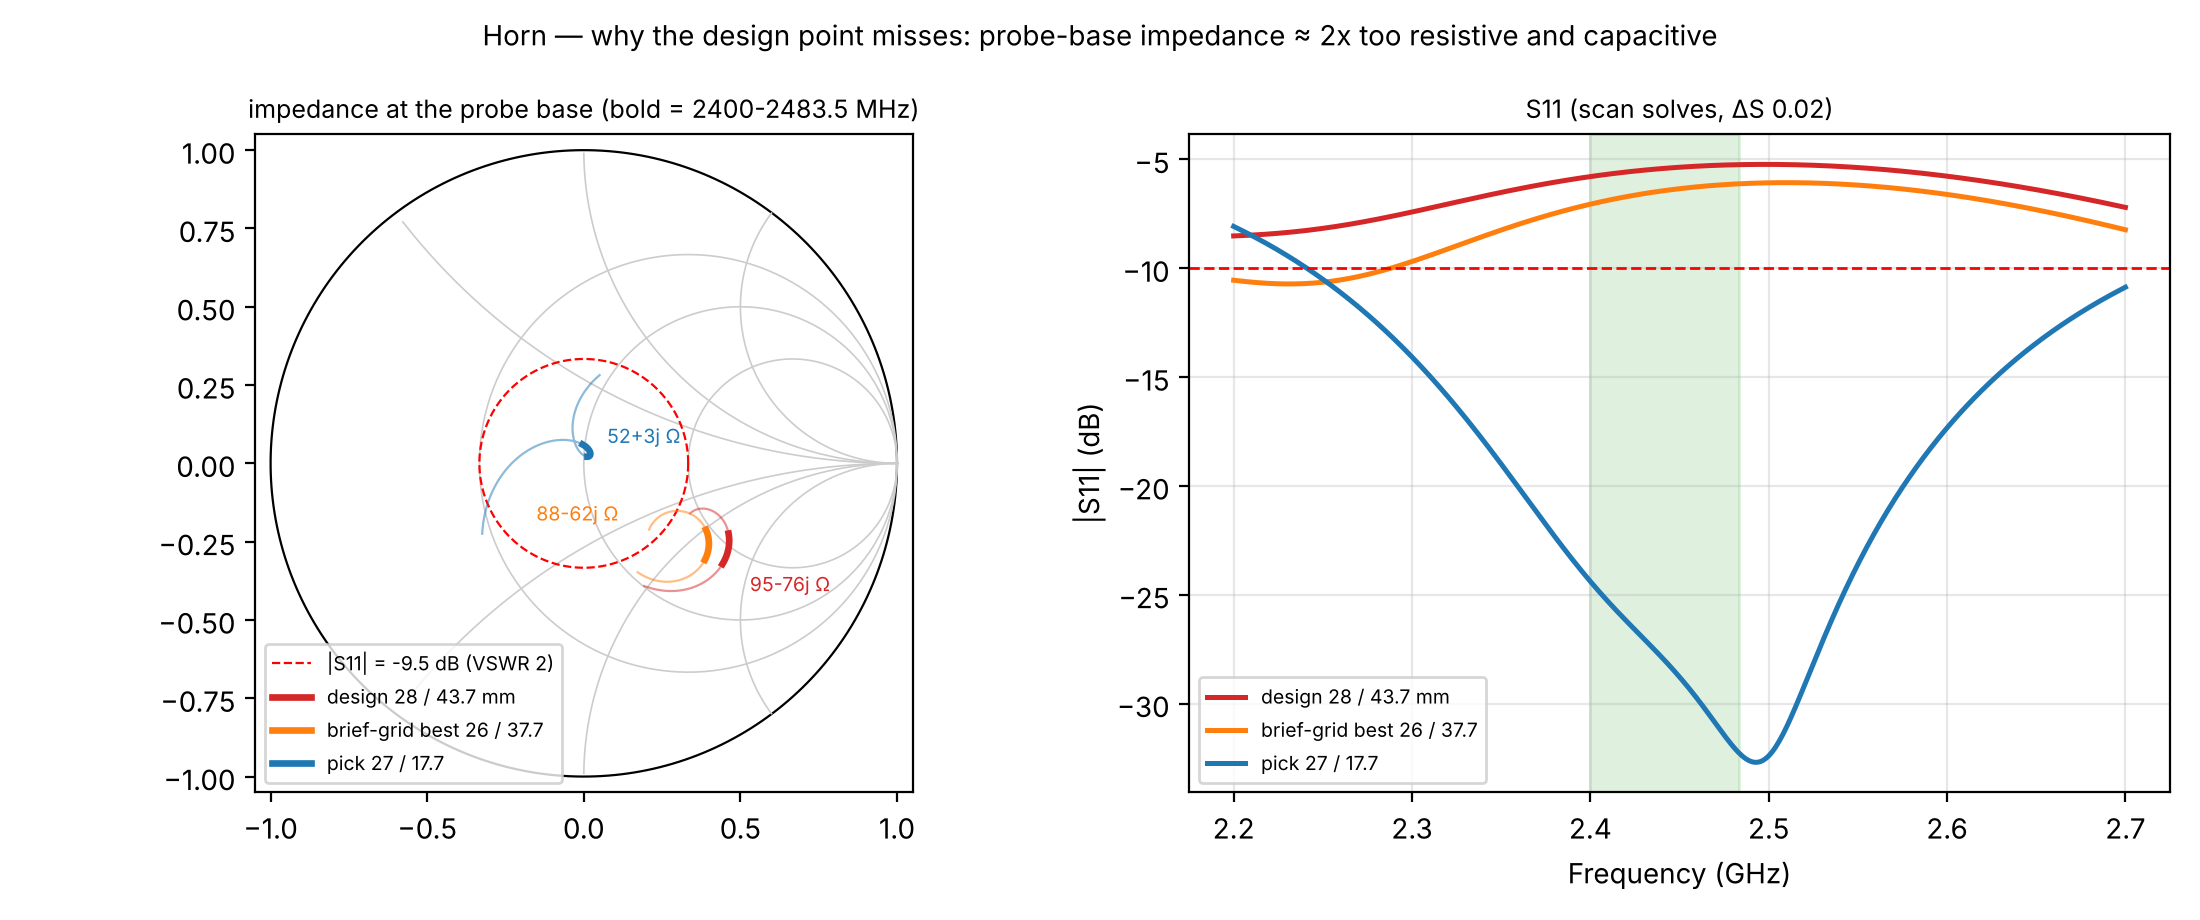
\includegraphics[width=0.85\linewidth,height=0.4\textheight,keepaspectratio]{figures/hfss/scan_diagnosis}\caption{Why the original probe position didn't match}\end{figure}
\begin{figure}[H]\centering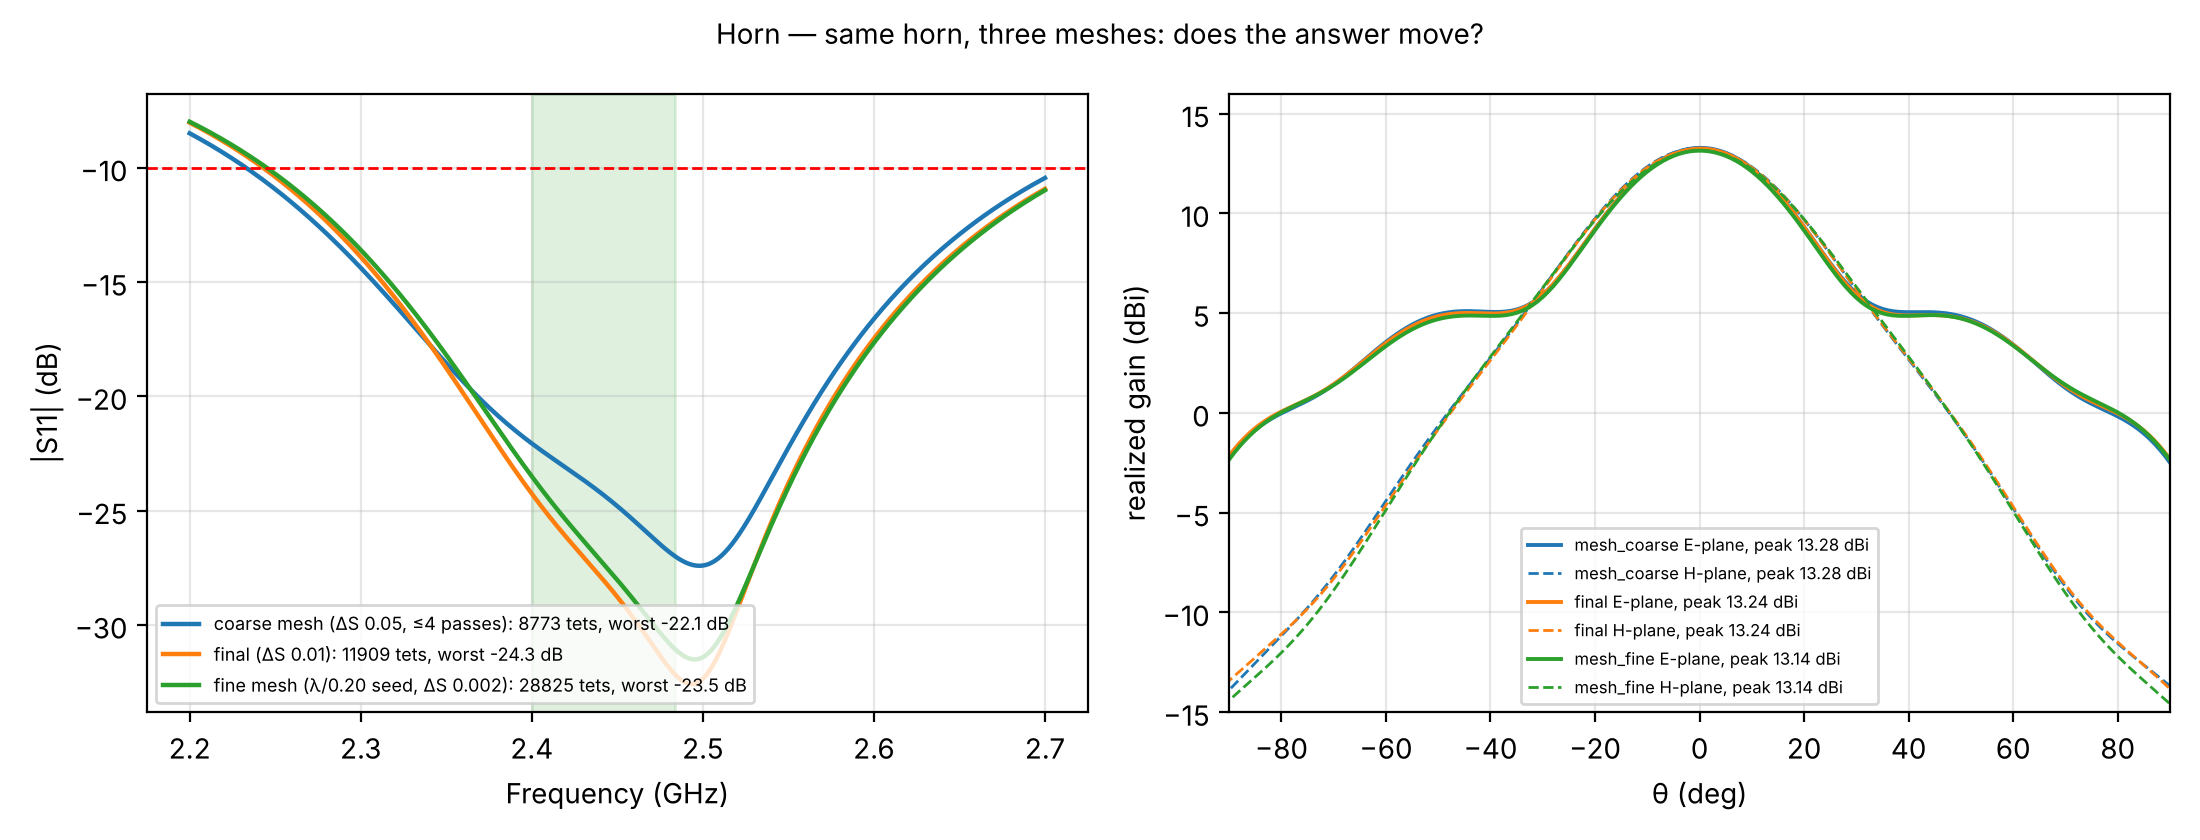
\includegraphics[width=0.85\linewidth,height=0.4\textheight,keepaspectratio]{figures/hfss/robust_mesh}\caption{Mesh check}\end{figure}
\begin{figure}[H]\centering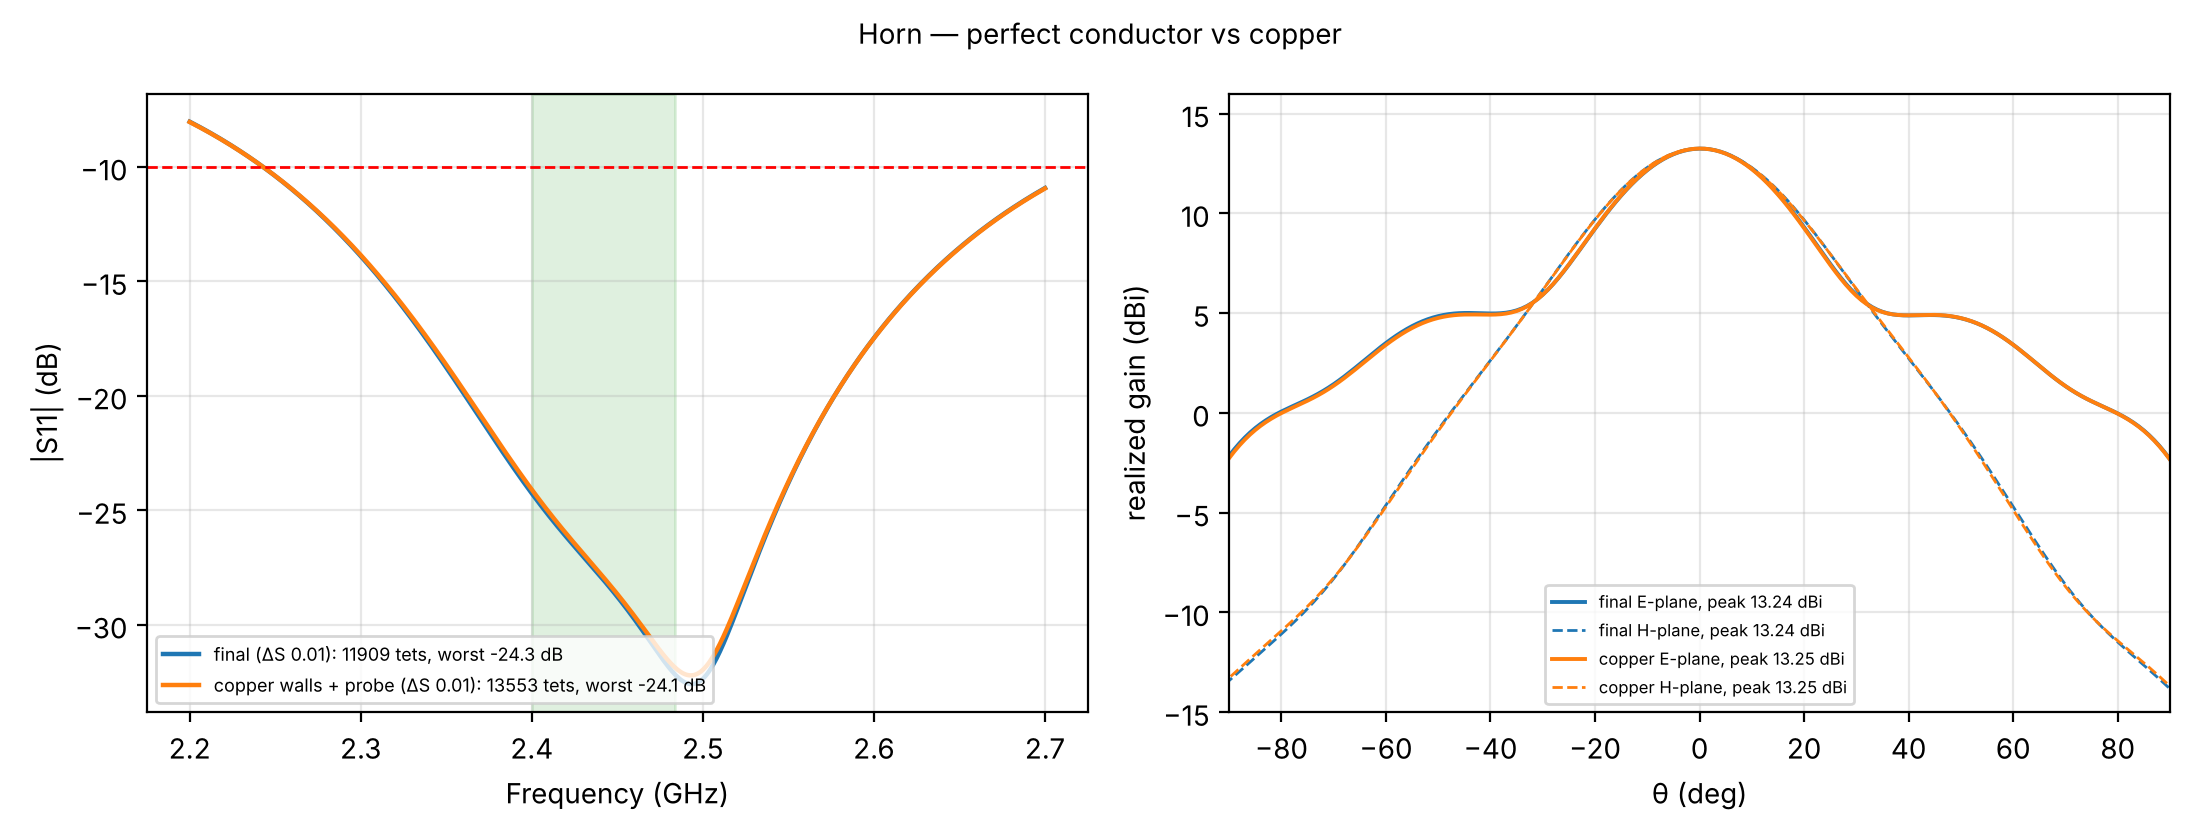
\includegraphics[width=0.85\linewidth,height=0.4\textheight,keepaspectratio]{figures/hfss/robust_copper}\caption{Copper vs. perfect conductor}\end{figure}
\begin{figure}[H]\centering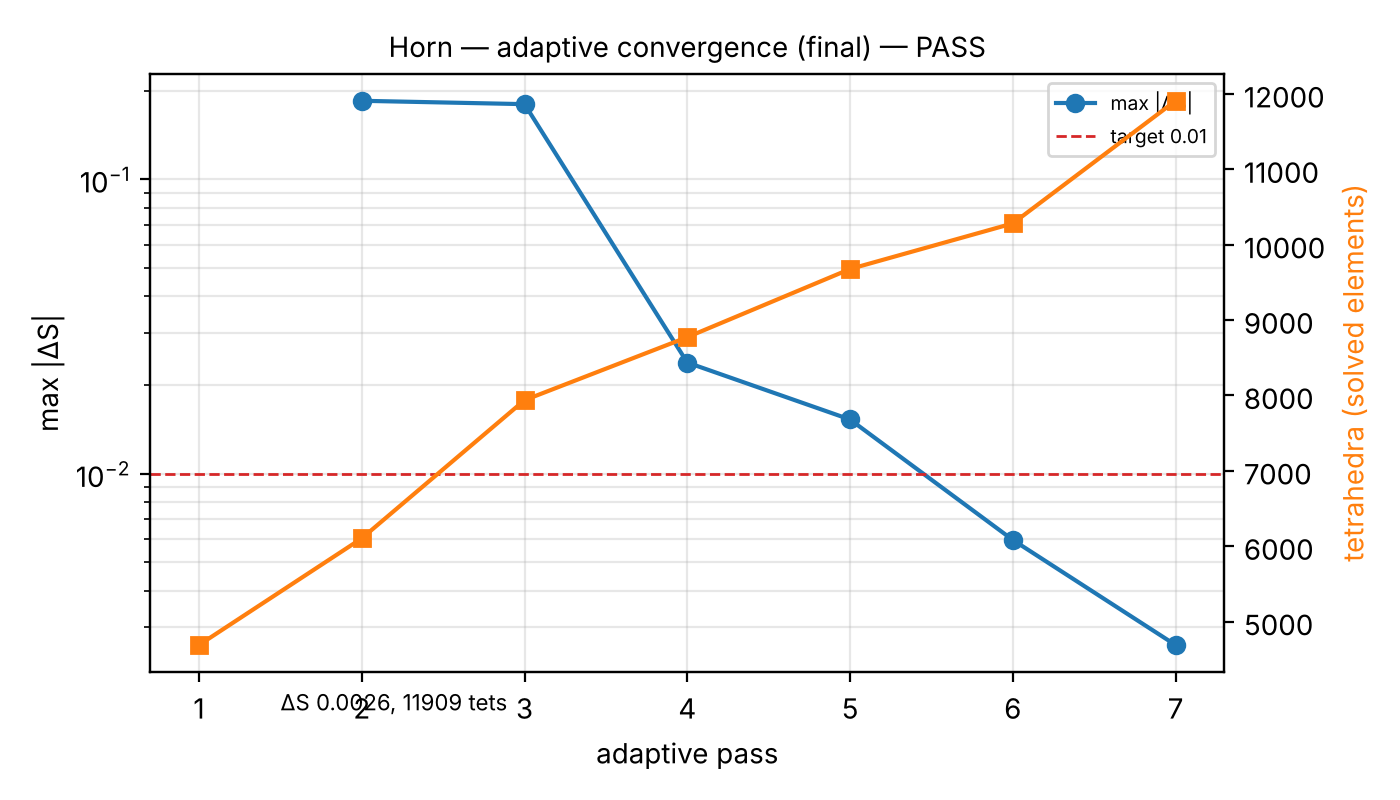
\includegraphics[width=0.85\linewidth,height=0.4\textheight,keepaspectratio]{figures/hfss/convergence}\caption{Mesh refinement}\end{figure}
\clearpage\subsection*{Baseband board (Multisim)}
\subsubsection*{Card 1: video amp}
\begin{figure}[H]\centering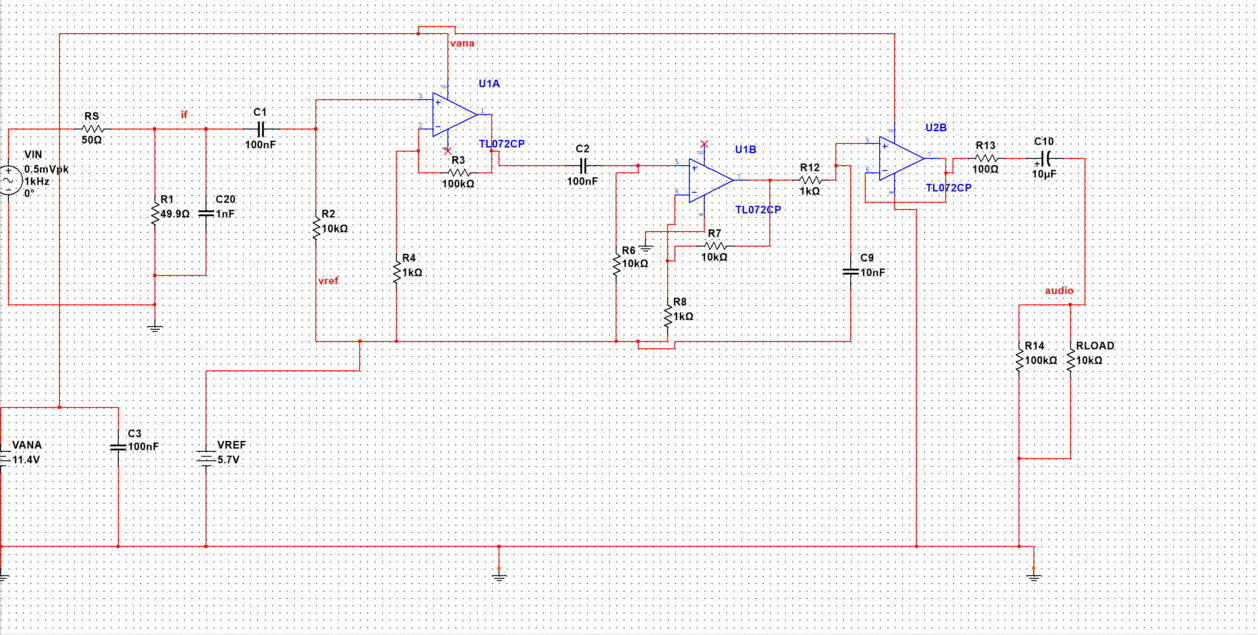
\includegraphics[width=0.85\linewidth,height=0.4\textheight,keepaspectratio]{figures/multisim/01_video_amp/01_schematic}\caption{Multisim schematic}\end{figure}
\begin{figure}[H]\centering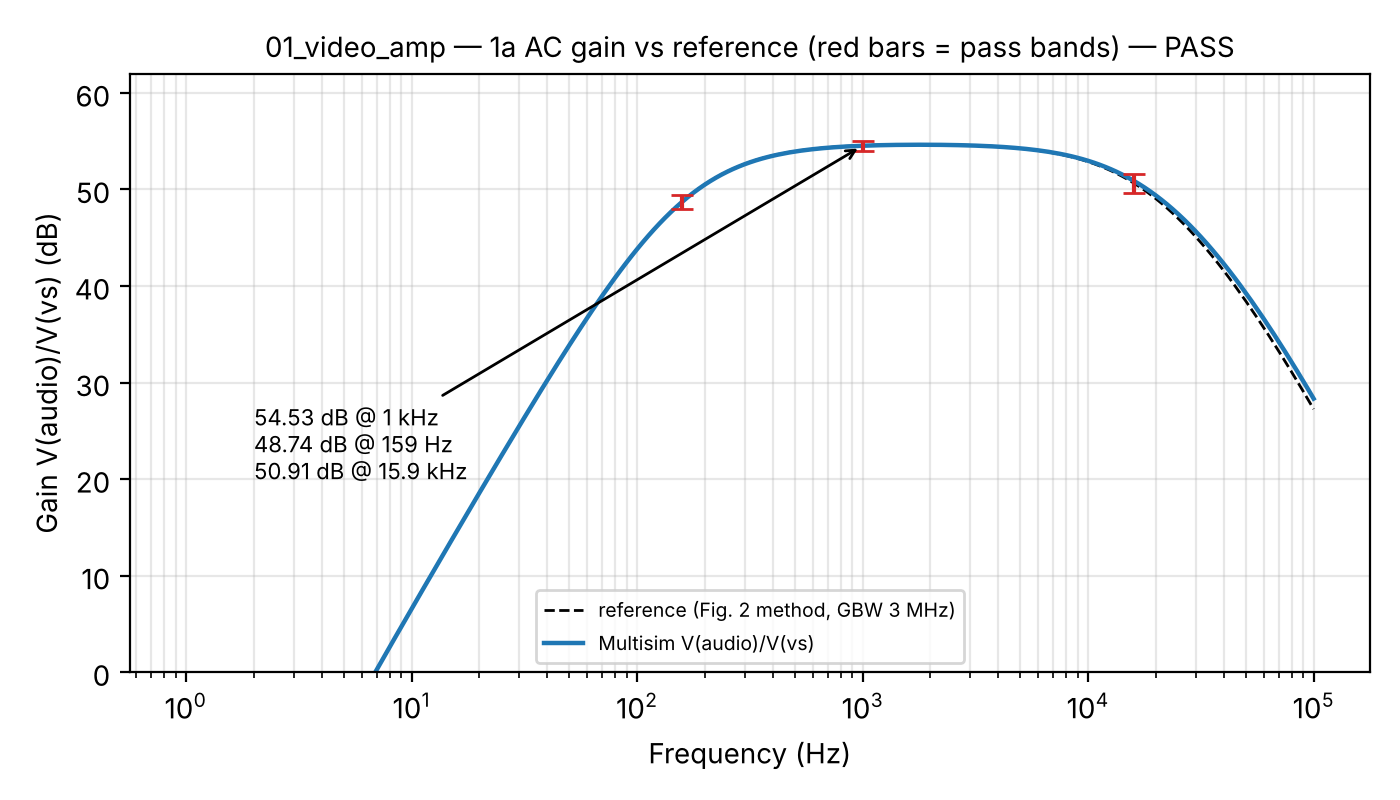
\includegraphics[width=0.85\linewidth,height=0.4\textheight,keepaspectratio]{figures/multisim/01_video_amp/01_bode}\caption{Gain vs. frequency}\end{figure}
\begin{figure}[H]\centering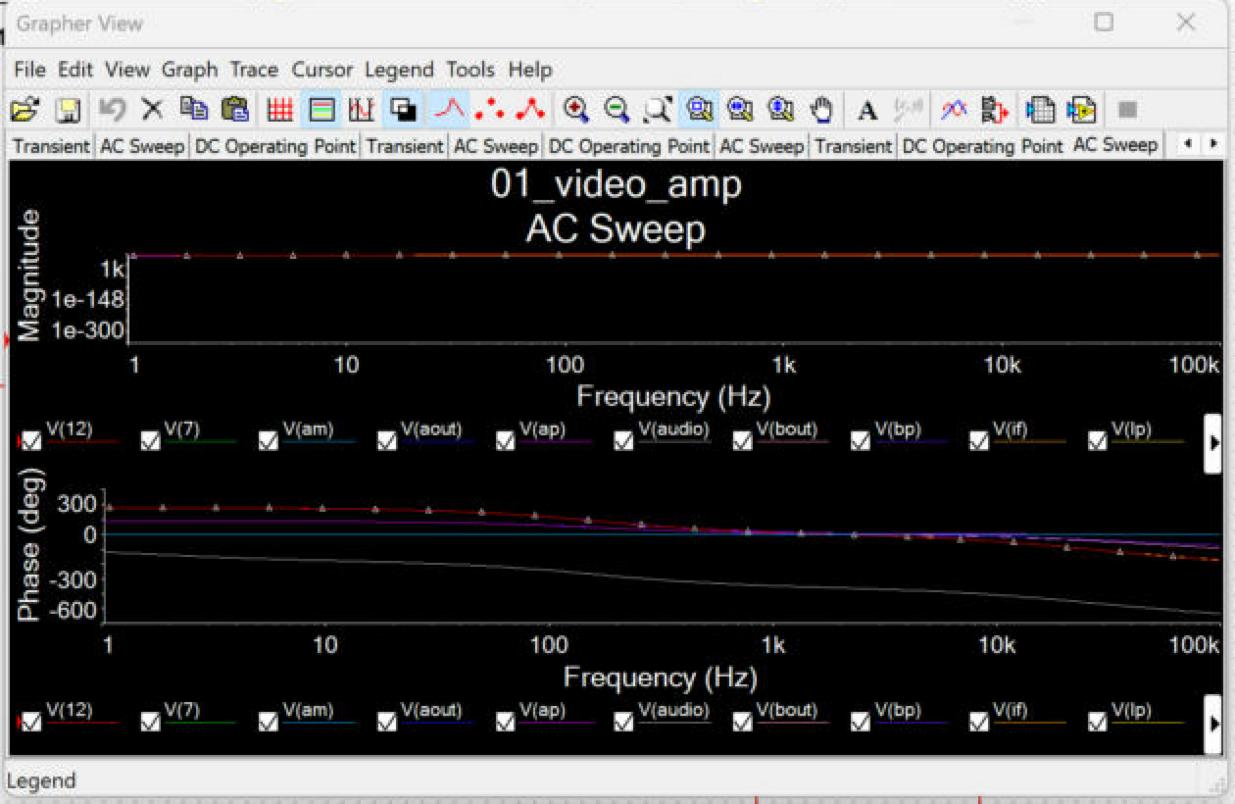
\includegraphics[width=0.85\linewidth,height=0.4\textheight,keepaspectratio]{figures/multisim/01_video_amp/01_grapher_ac}\caption{Multisim grapher, AC sweep}\end{figure}
\begin{figure}[H]\centering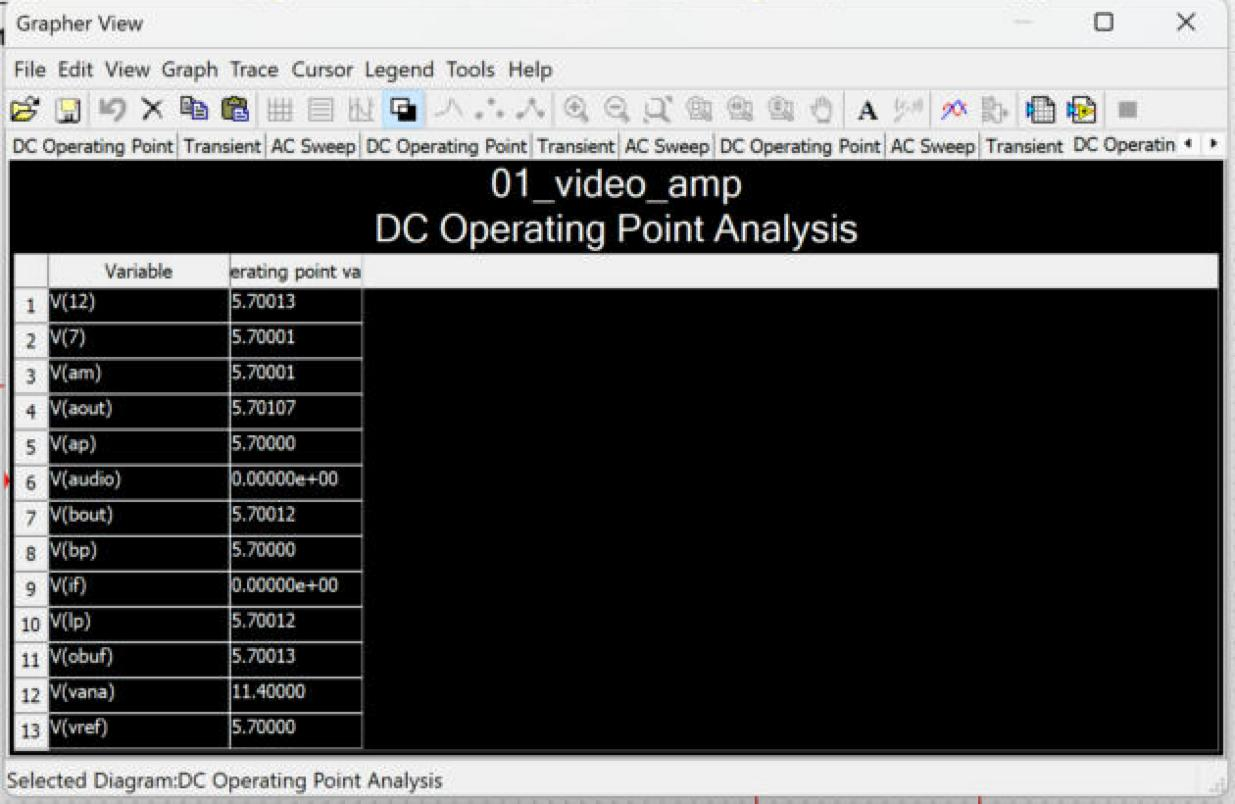
\includegraphics[width=0.85\linewidth,height=0.4\textheight,keepaspectratio]{figures/multisim/01_video_amp/01_grapher_dcop}\caption{Multisim grapher, DC operating point}\end{figure}
\begin{figure}[H]\centering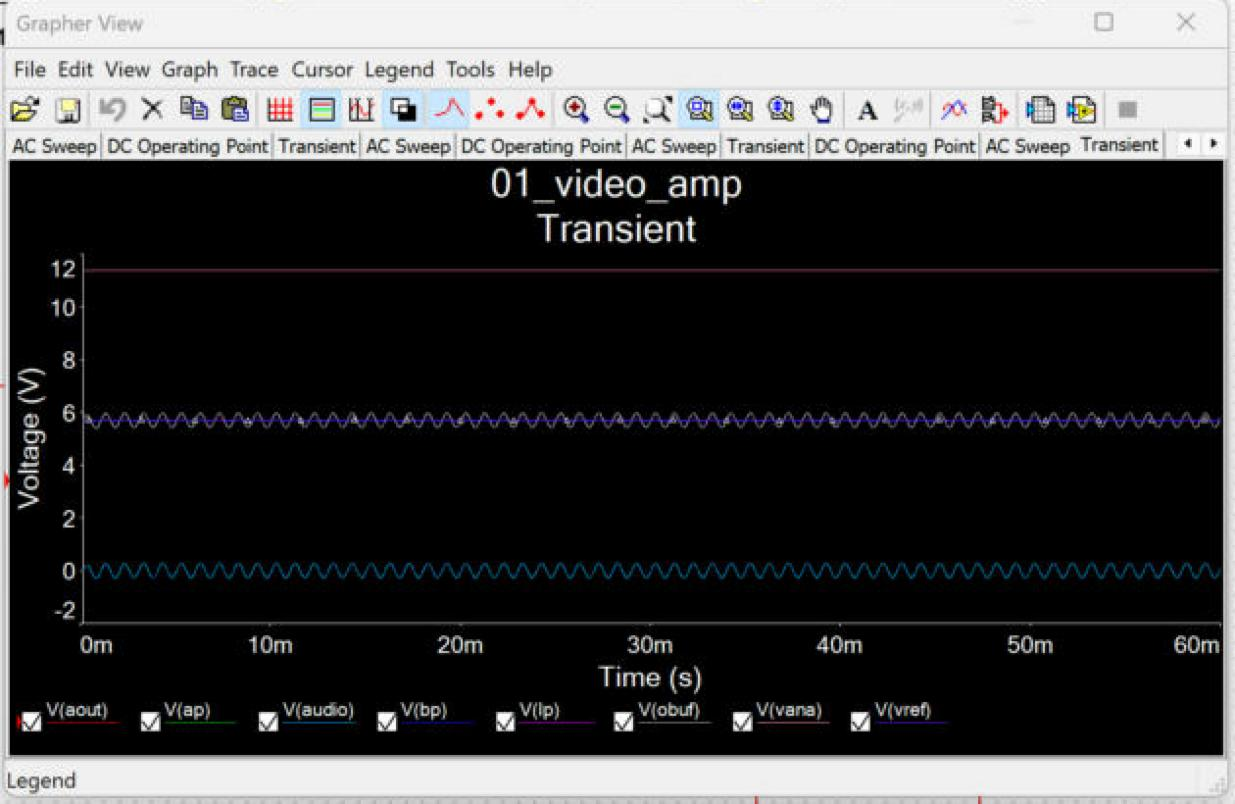
\includegraphics[width=0.85\linewidth,height=0.4\textheight,keepaspectratio]{figures/multisim/01_video_amp/01_grapher_tran}\caption{Multisim grapher, transient}\end{figure}
\begin{figure}[H]\centering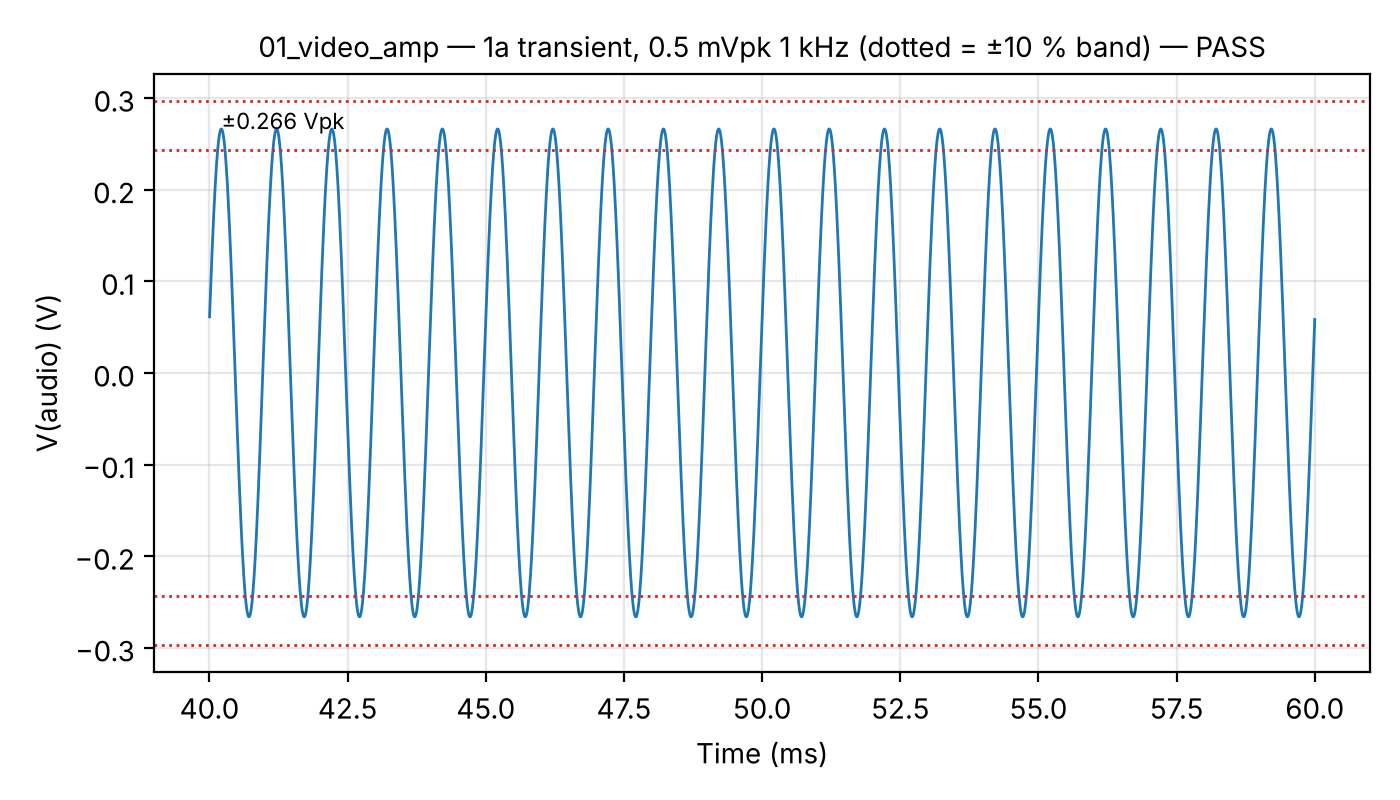
\includegraphics[width=0.85\linewidth,height=0.4\textheight,keepaspectratio]{figures/multisim/01_video_amp/01_tran}\caption{1 kHz transient}\end{figure}
\begin{figure}[H]\centering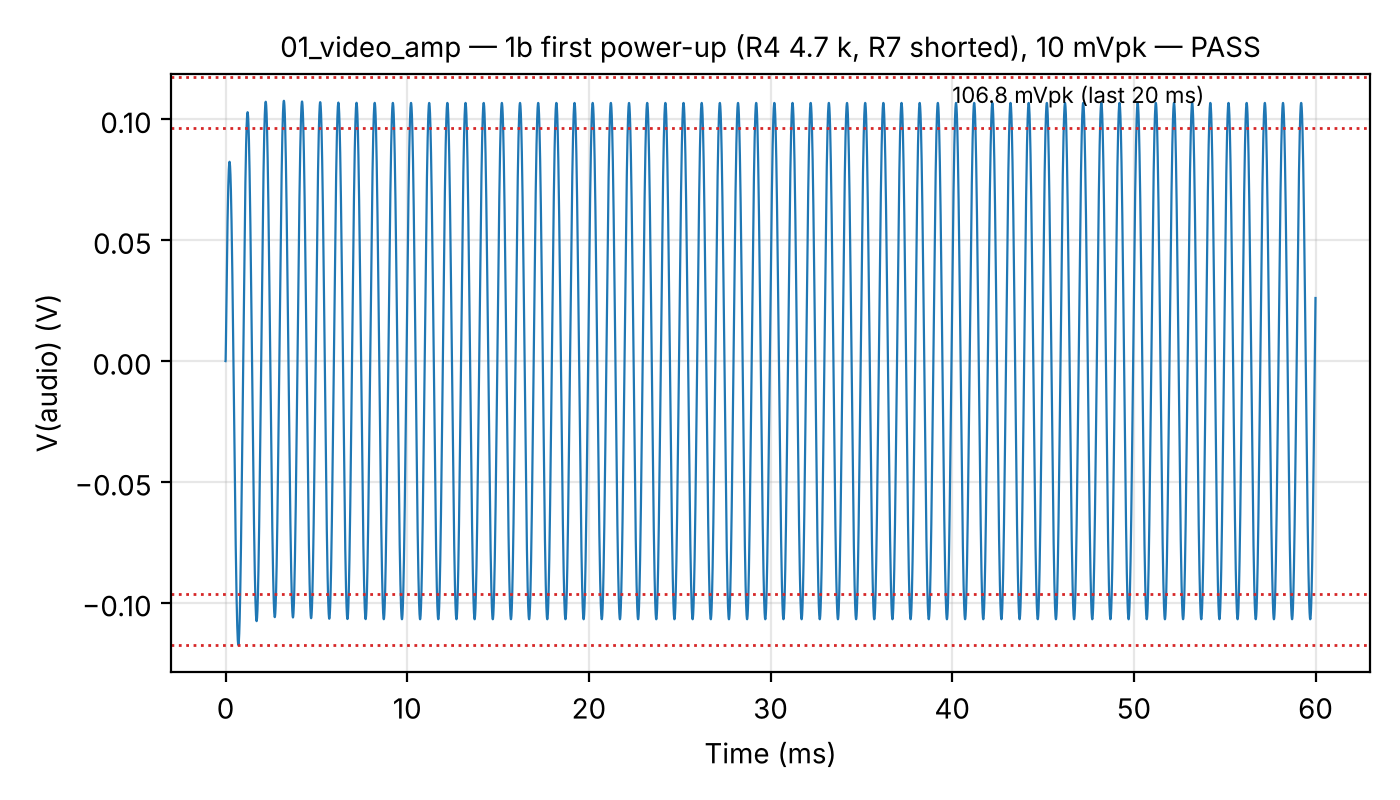
\includegraphics[width=0.85\linewidth,height=0.4\textheight,keepaspectratio]{figures/multisim/01_video_amp/01b_powerup}\caption{First power-up gain}\end{figure}
\begin{figure}[H]\centering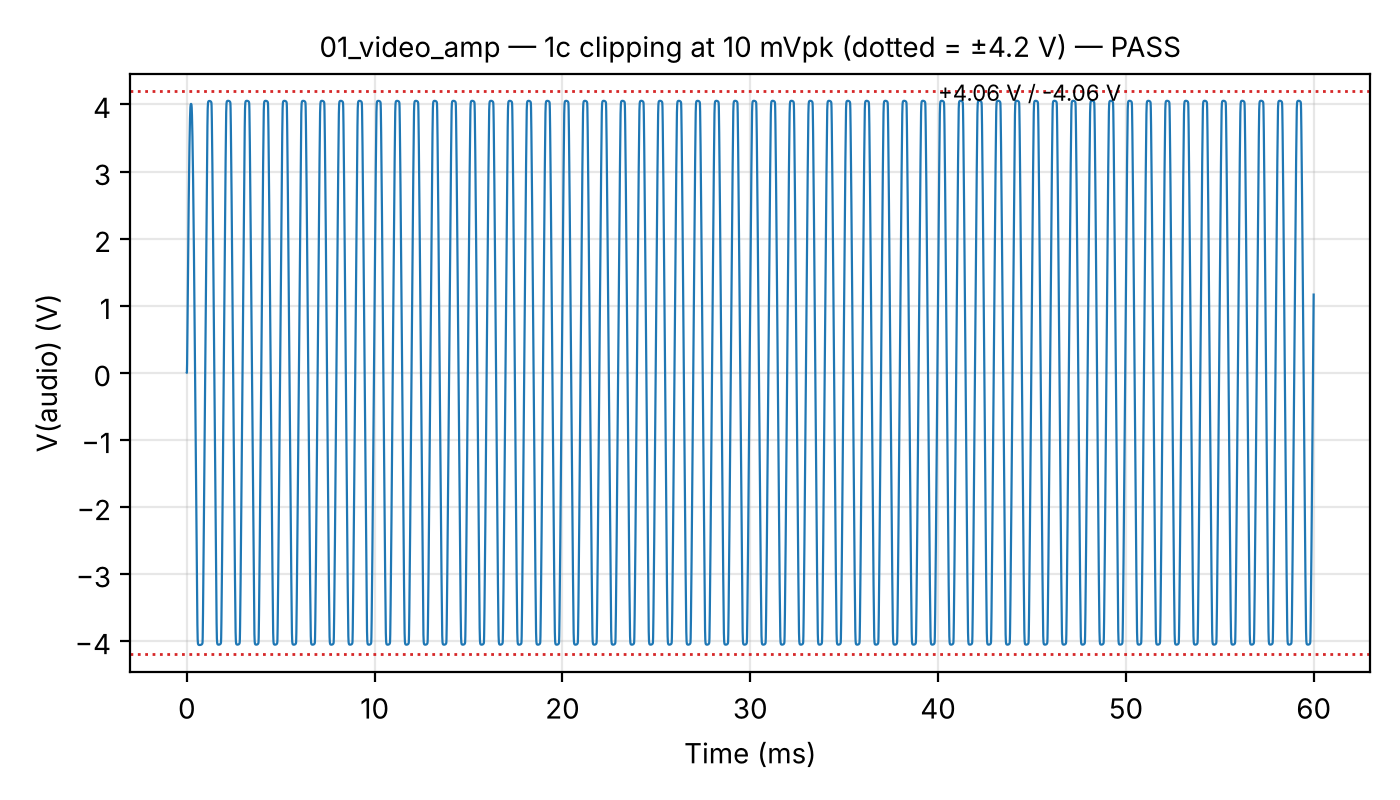
\includegraphics[width=0.85\linewidth,height=0.4\textheight,keepaspectratio]{figures/multisim/01_video_amp/01c_clipping}\caption{Clipping at 10 mV in}\end{figure}
\begin{figure}[H]\centering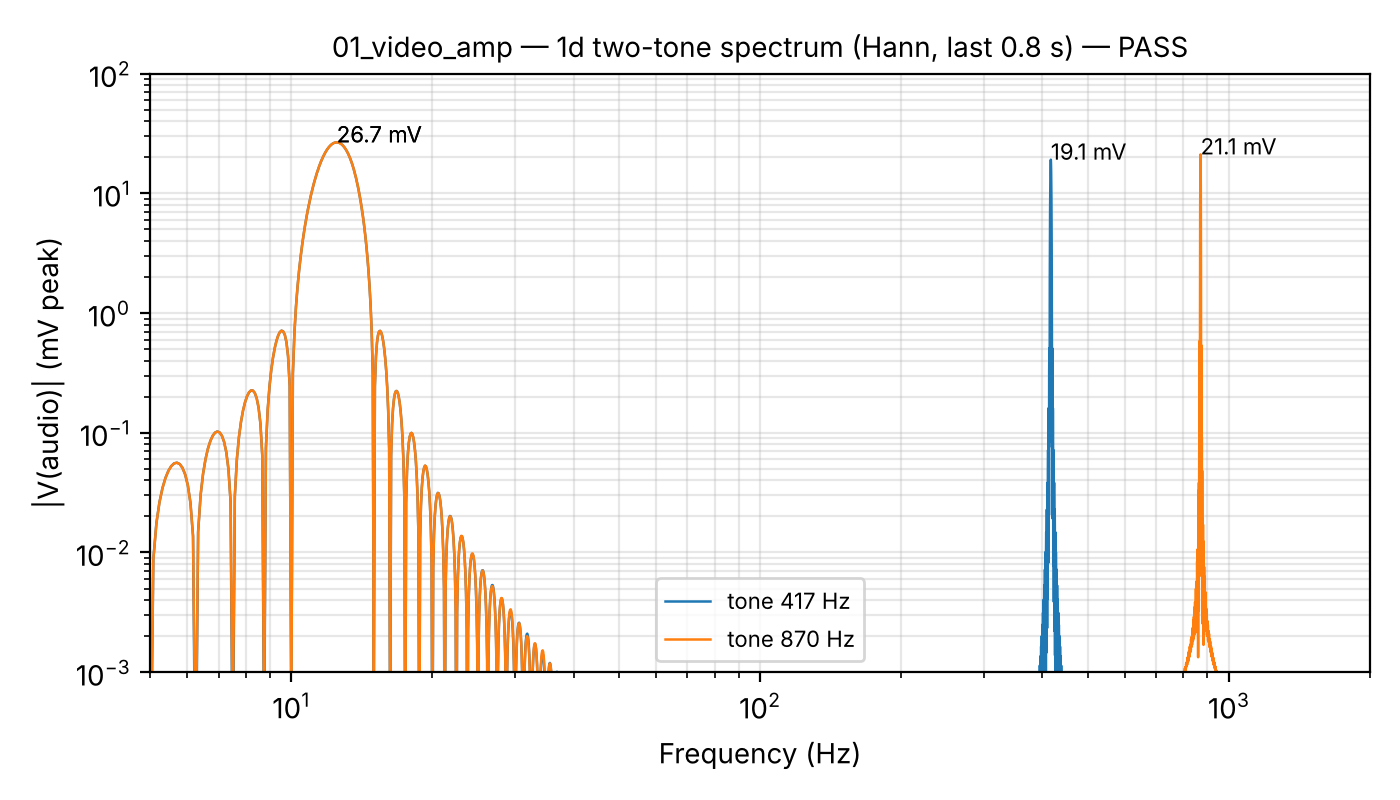
\includegraphics[width=0.85\linewidth,height=0.4\textheight,keepaspectratio]{figures/multisim/01_video_amp/01d_twotone_spectrum}\caption{Two-tone spectrum (leakage + echo)}\end{figure}
\clearpage
\subsubsection*{Card 2: half-rail reference}
\begin{figure}[H]\centering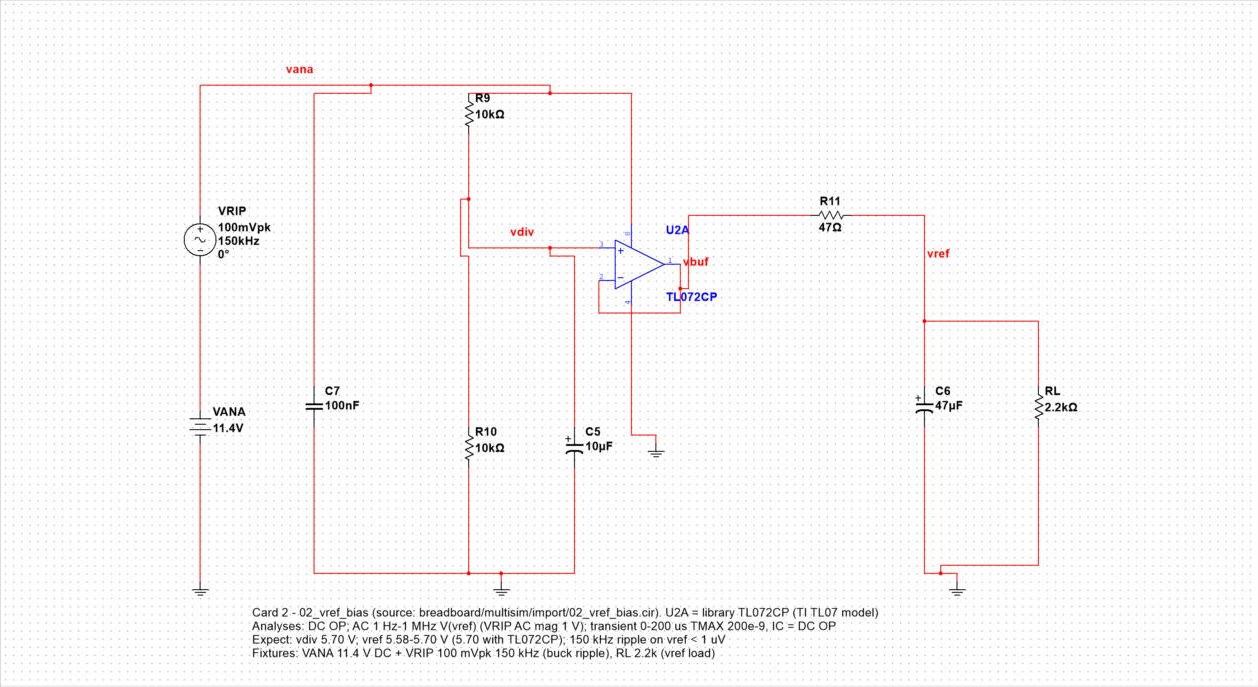
\includegraphics[width=0.85\linewidth,height=0.4\textheight,keepaspectratio]{figures/multisim/02_vref_bias/02_schematic}\caption{Multisim schematic}\end{figure}
\begin{figure}[H]\centering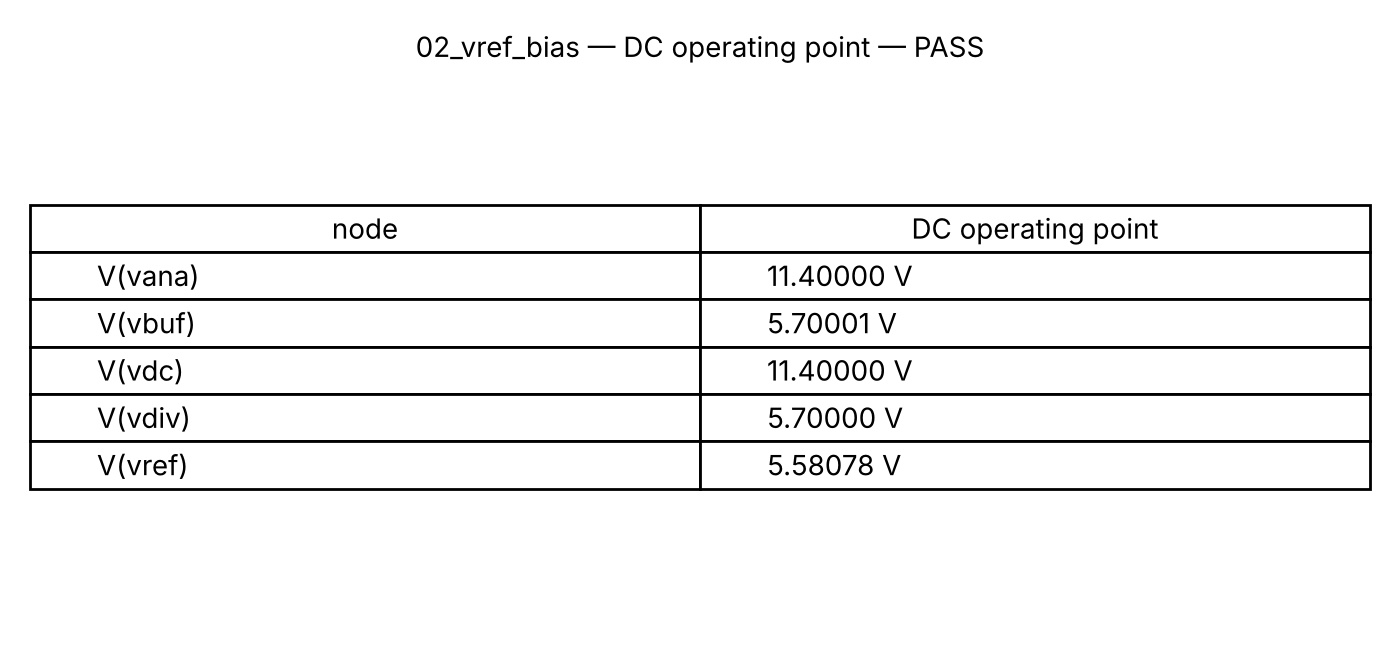
\includegraphics[width=0.85\linewidth,height=0.4\textheight,keepaspectratio]{figures/multisim/02_vref_bias/02_dc_table}\caption{DC operating point}\end{figure}
\begin{figure}[H]\centering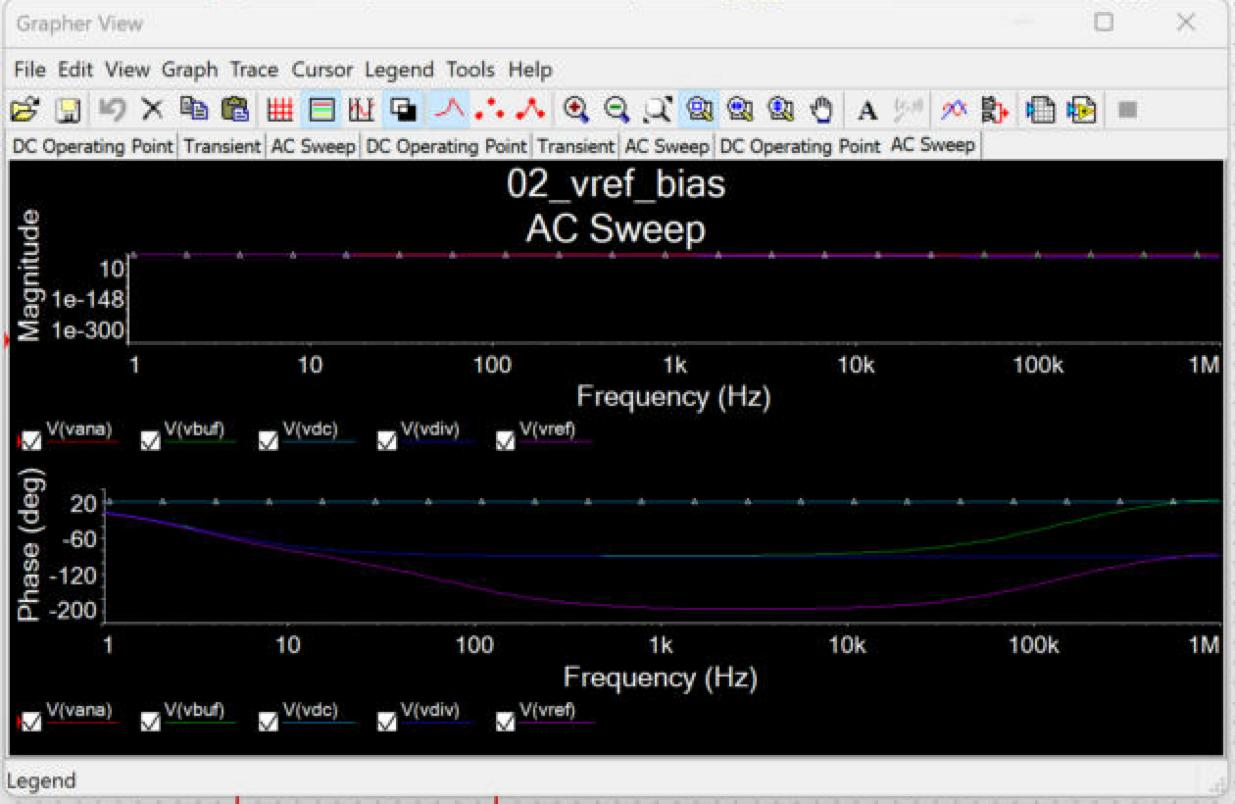
\includegraphics[width=0.85\linewidth,height=0.4\textheight,keepaspectratio]{figures/multisim/02_vref_bias/02_grapher_ac}\caption{Multisim grapher, AC sweep}\end{figure}
\begin{figure}[H]\centering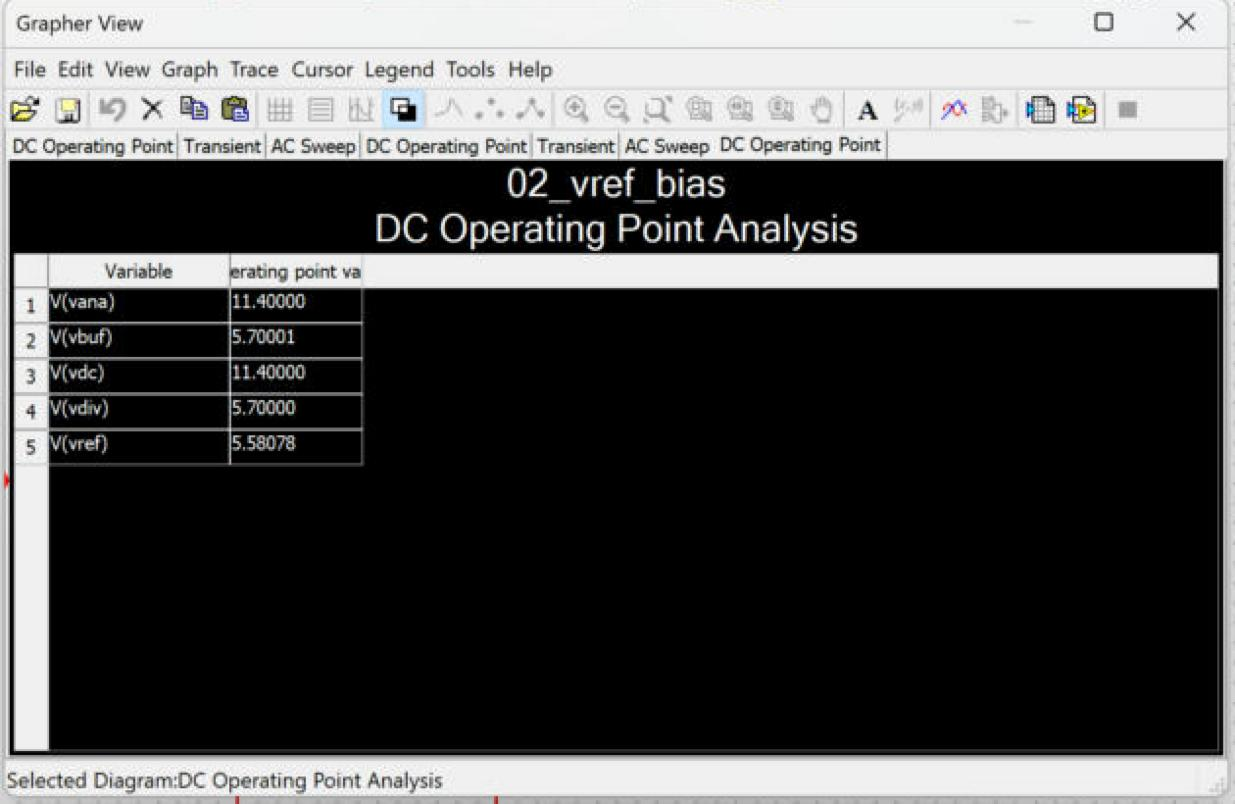
\includegraphics[width=0.85\linewidth,height=0.4\textheight,keepaspectratio]{figures/multisim/02_vref_bias/02_grapher_dcop}\caption{Multisim grapher, DC operating point}\end{figure}
\begin{figure}[H]\centering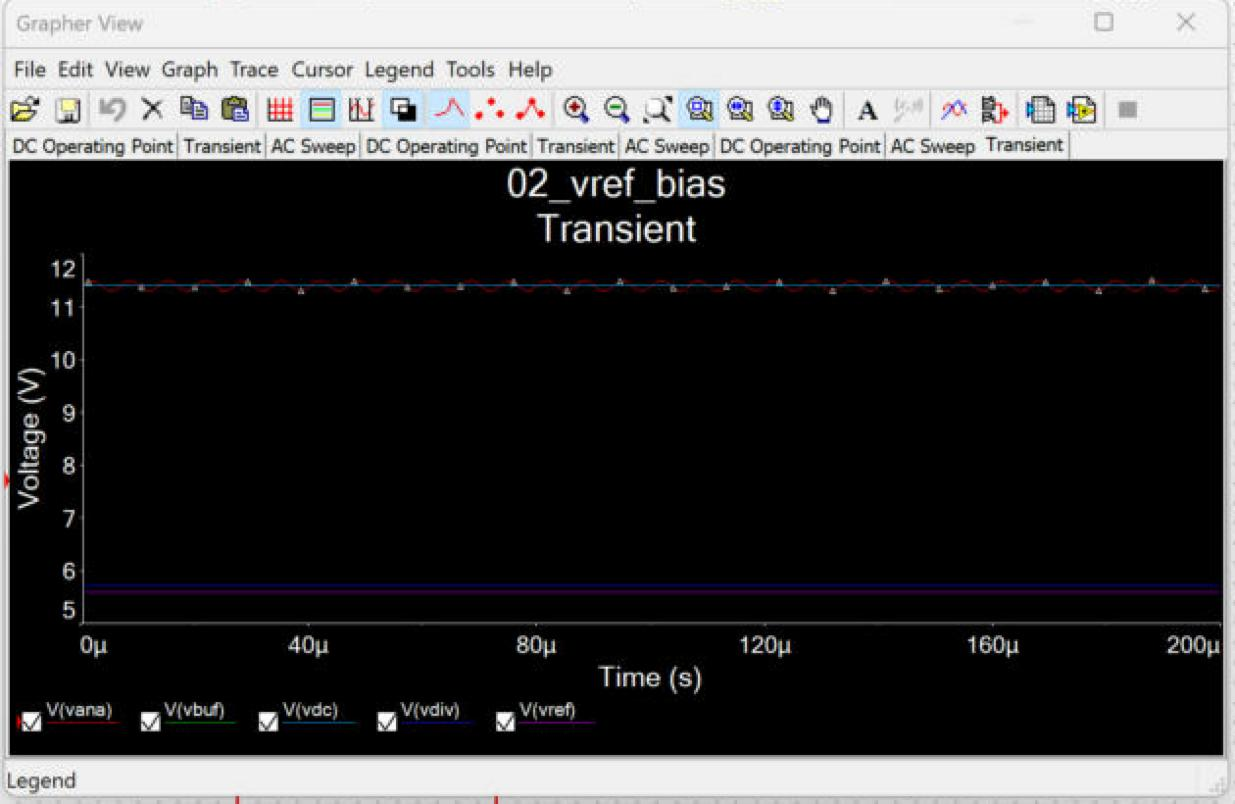
\includegraphics[width=0.85\linewidth,height=0.4\textheight,keepaspectratio]{figures/multisim/02_vref_bias/02_grapher_tran}\caption{Multisim grapher, transient}\end{figure}
\begin{figure}[H]\centering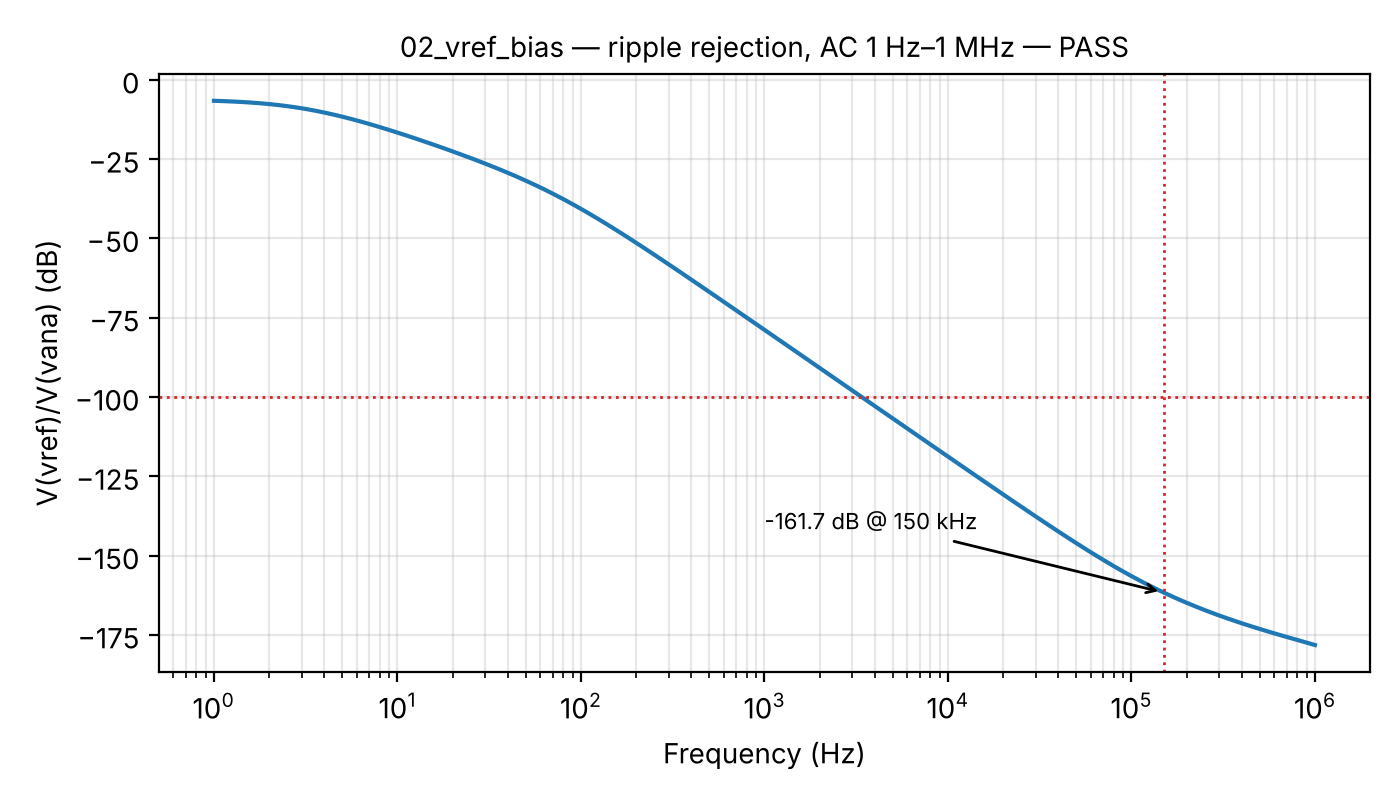
\includegraphics[width=0.85\linewidth,height=0.4\textheight,keepaspectratio]{figures/multisim/02_vref_bias/02_rejection}\caption{150 kHz rejection to vref}\end{figure}
\begin{figure}[H]\centering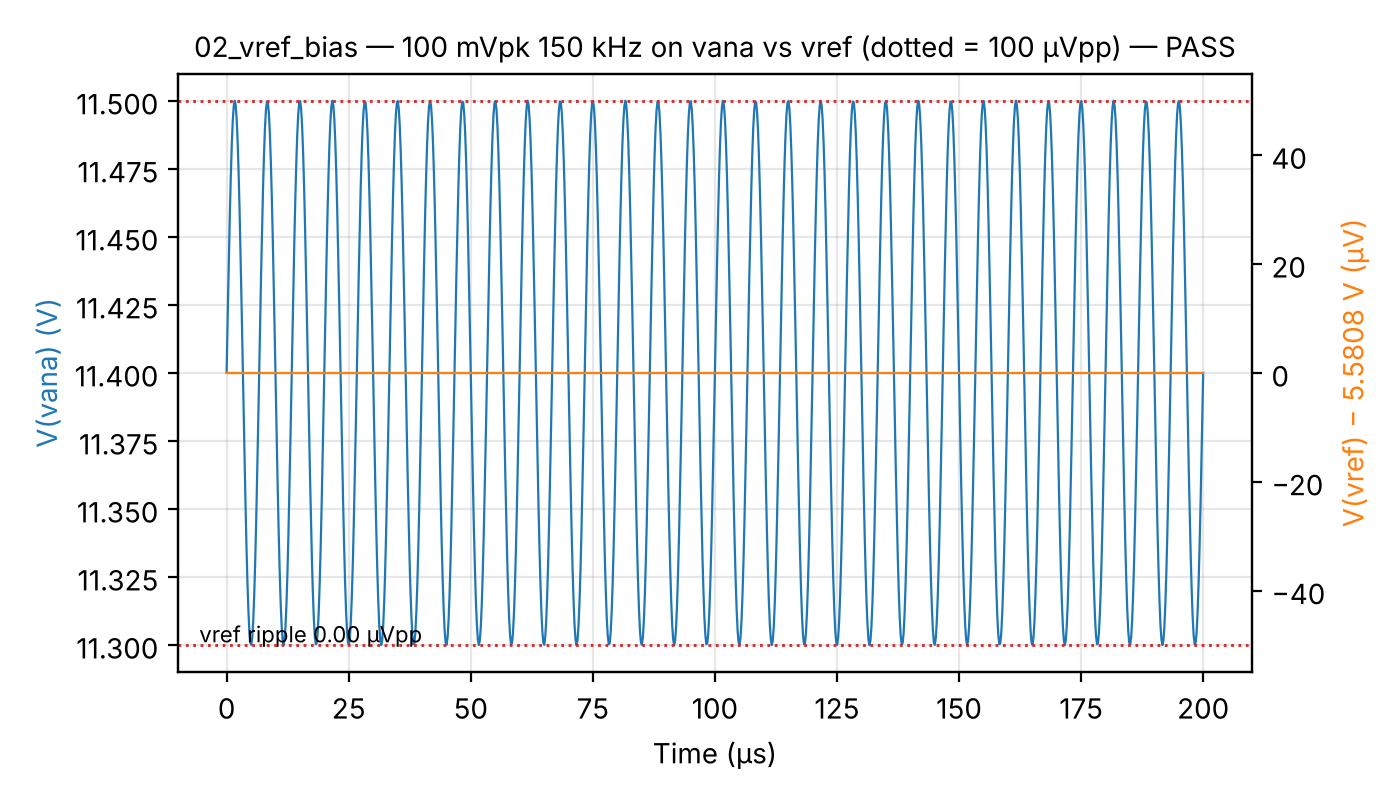
\includegraphics[width=0.85\linewidth,height=0.4\textheight,keepaspectratio]{figures/multisim/02_vref_bias/02_ripple}\caption{Ripple on vref}\end{figure}
\clearpage
\subsubsection*{Card 3: 12 V input}
\begin{figure}[H]\centering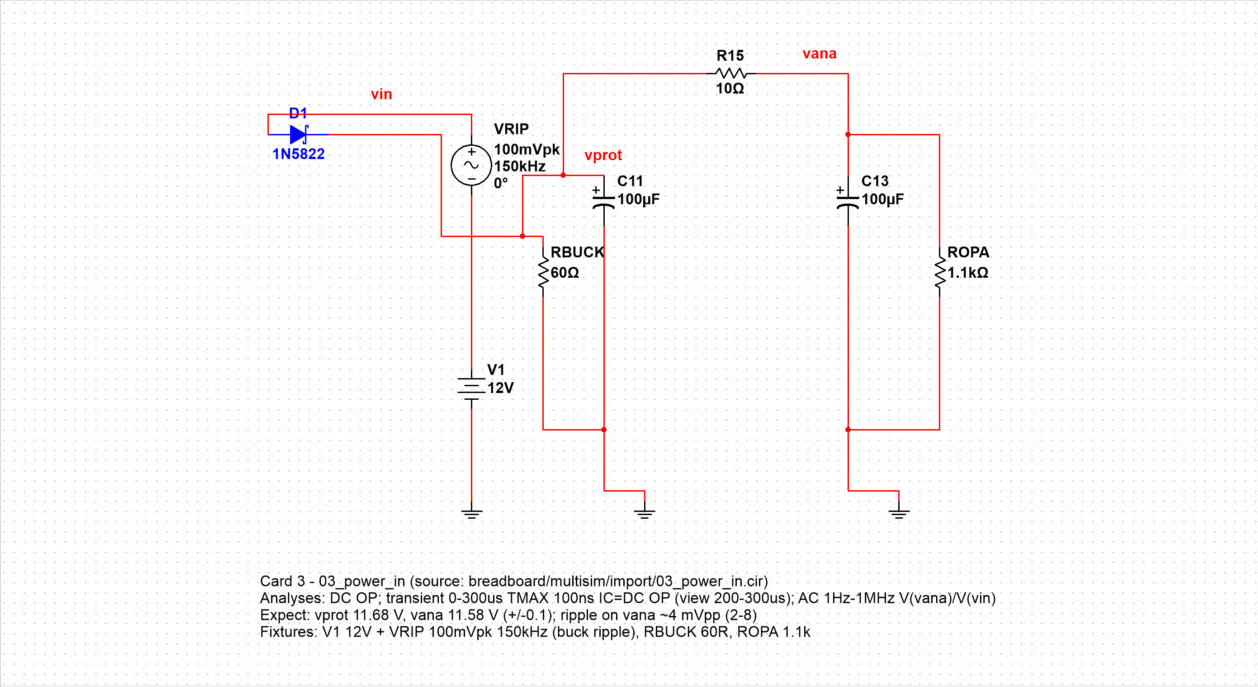
\includegraphics[width=0.85\linewidth,height=0.4\textheight,keepaspectratio]{figures/multisim/03_power_in/03_schematic}\caption{Multisim schematic}\end{figure}
\begin{figure}[H]\centering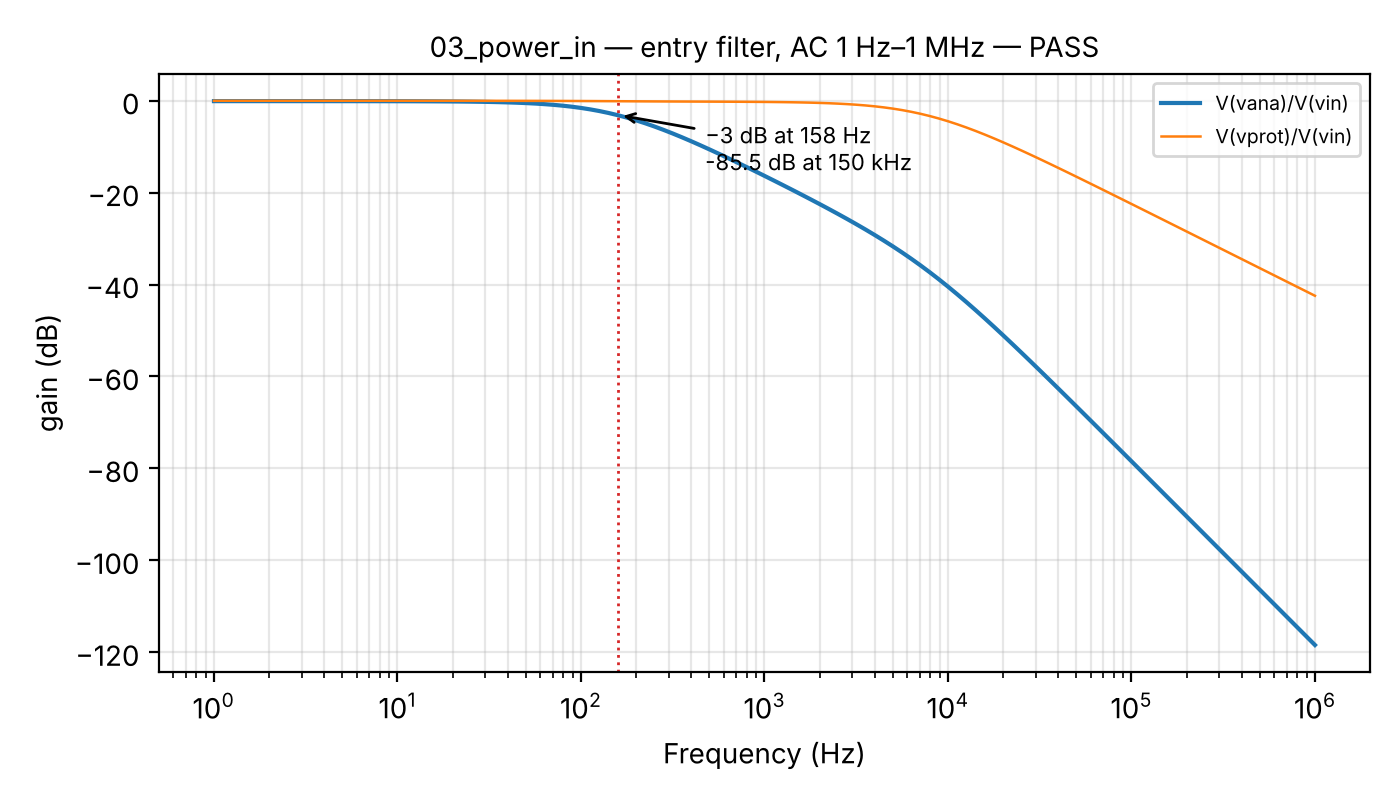
\includegraphics[width=0.85\linewidth,height=0.4\textheight,keepaspectratio]{figures/multisim/03_power_in/03_ac_filter}\caption{Input filter response}\end{figure}
\begin{figure}[H]\centering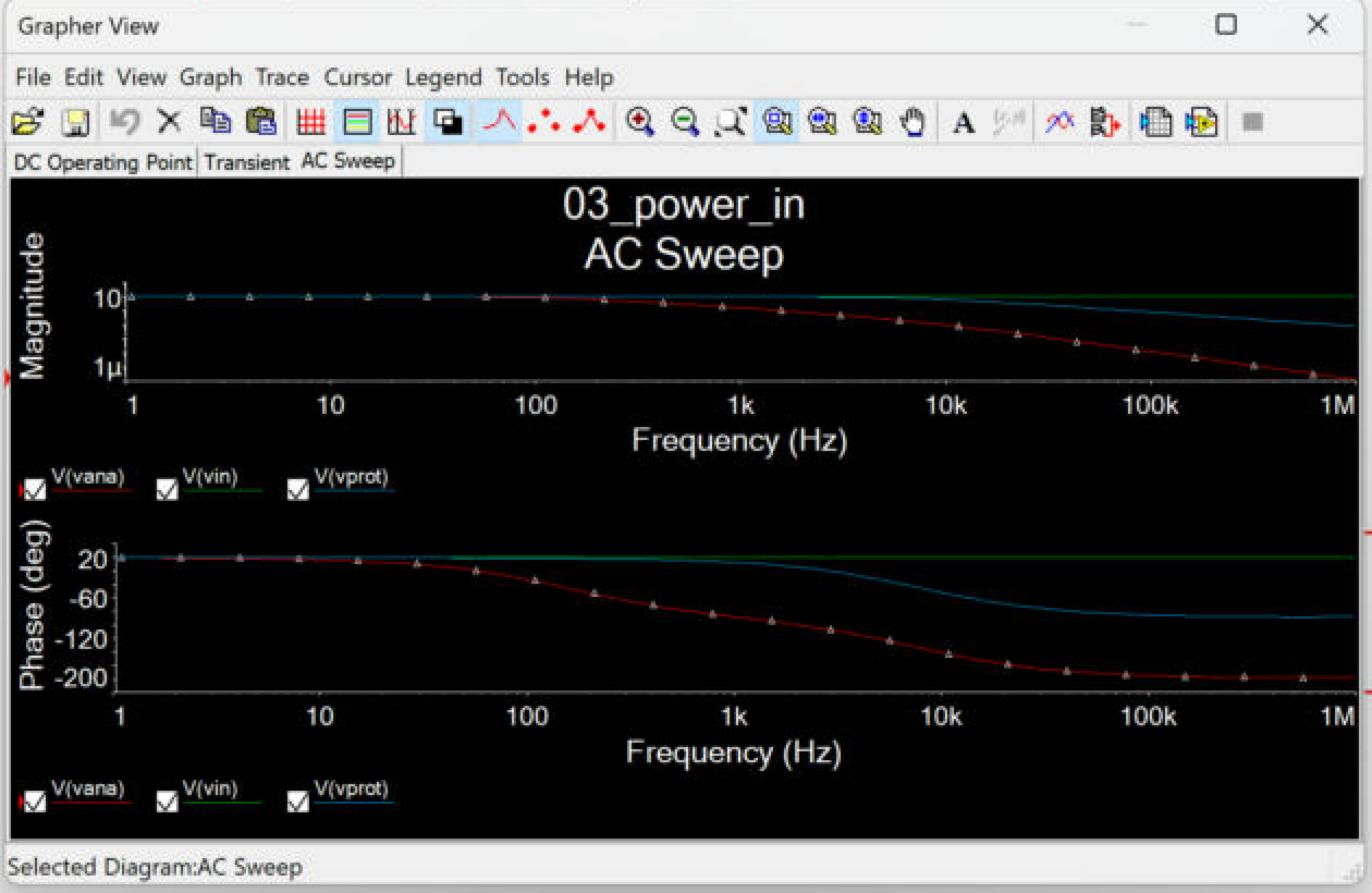
\includegraphics[width=0.85\linewidth,height=0.4\textheight,keepaspectratio]{figures/multisim/03_power_in/03_grapher_ac}\caption{Multisim grapher, AC sweep}\end{figure}
\begin{figure}[H]\centering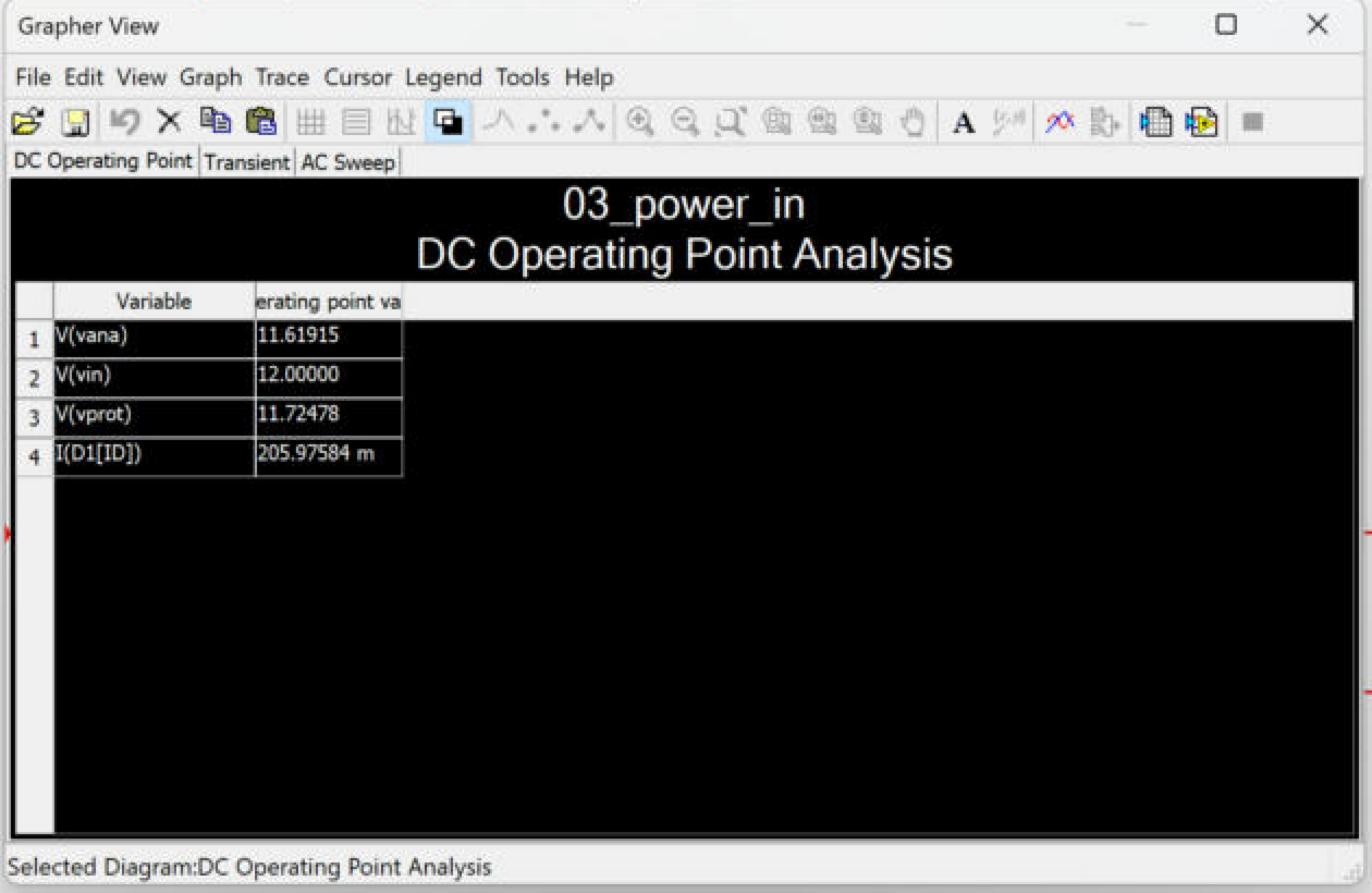
\includegraphics[width=0.85\linewidth,height=0.4\textheight,keepaspectratio]{figures/multisim/03_power_in/03_grapher_dcop}\caption{Multisim grapher, DC operating point}\end{figure}
\begin{figure}[H]\centering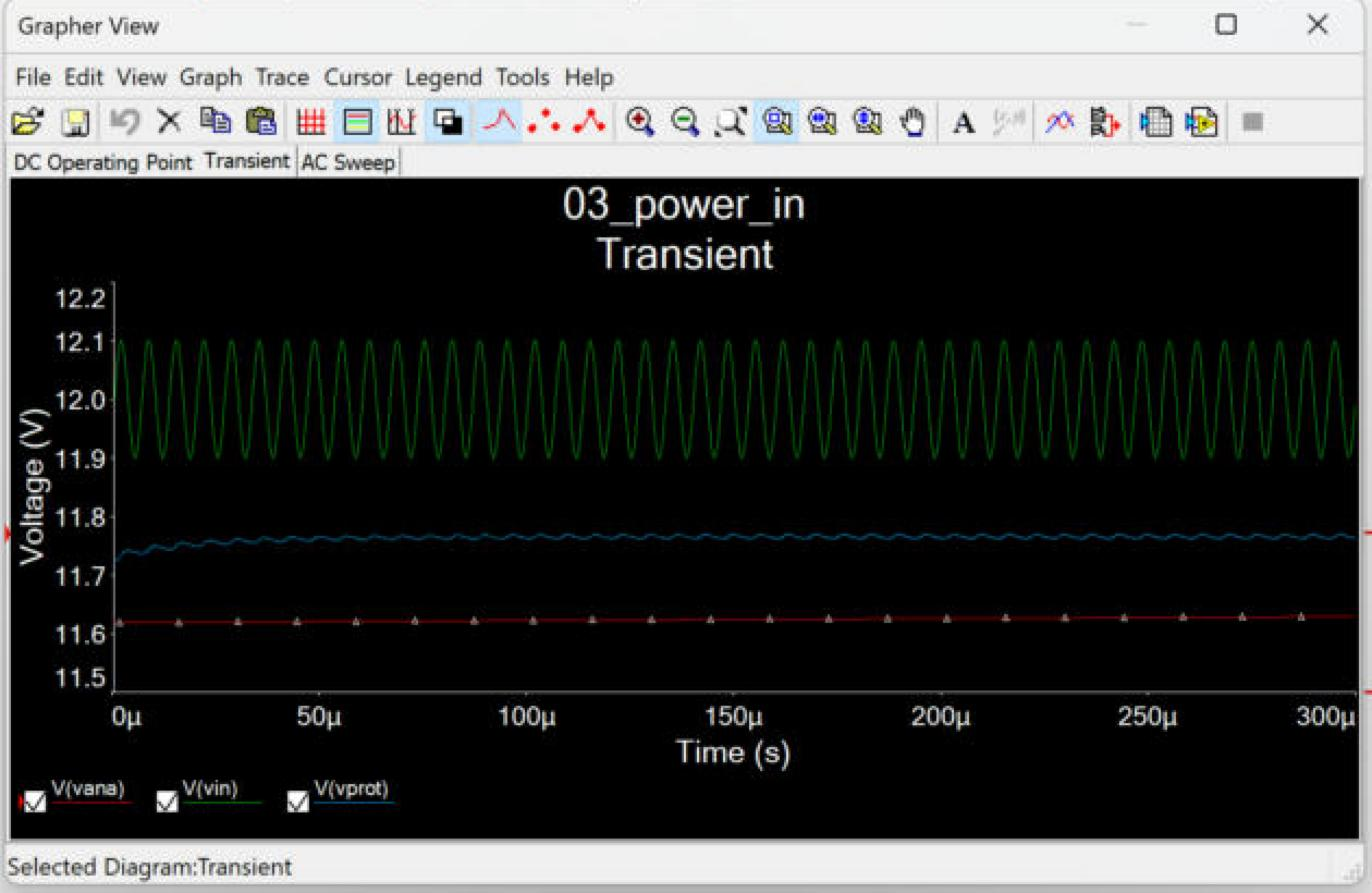
\includegraphics[width=0.85\linewidth,height=0.4\textheight,keepaspectratio]{figures/multisim/03_power_in/03_grapher_tran}\caption{Multisim grapher, transient}\end{figure}
\begin{figure}[H]\centering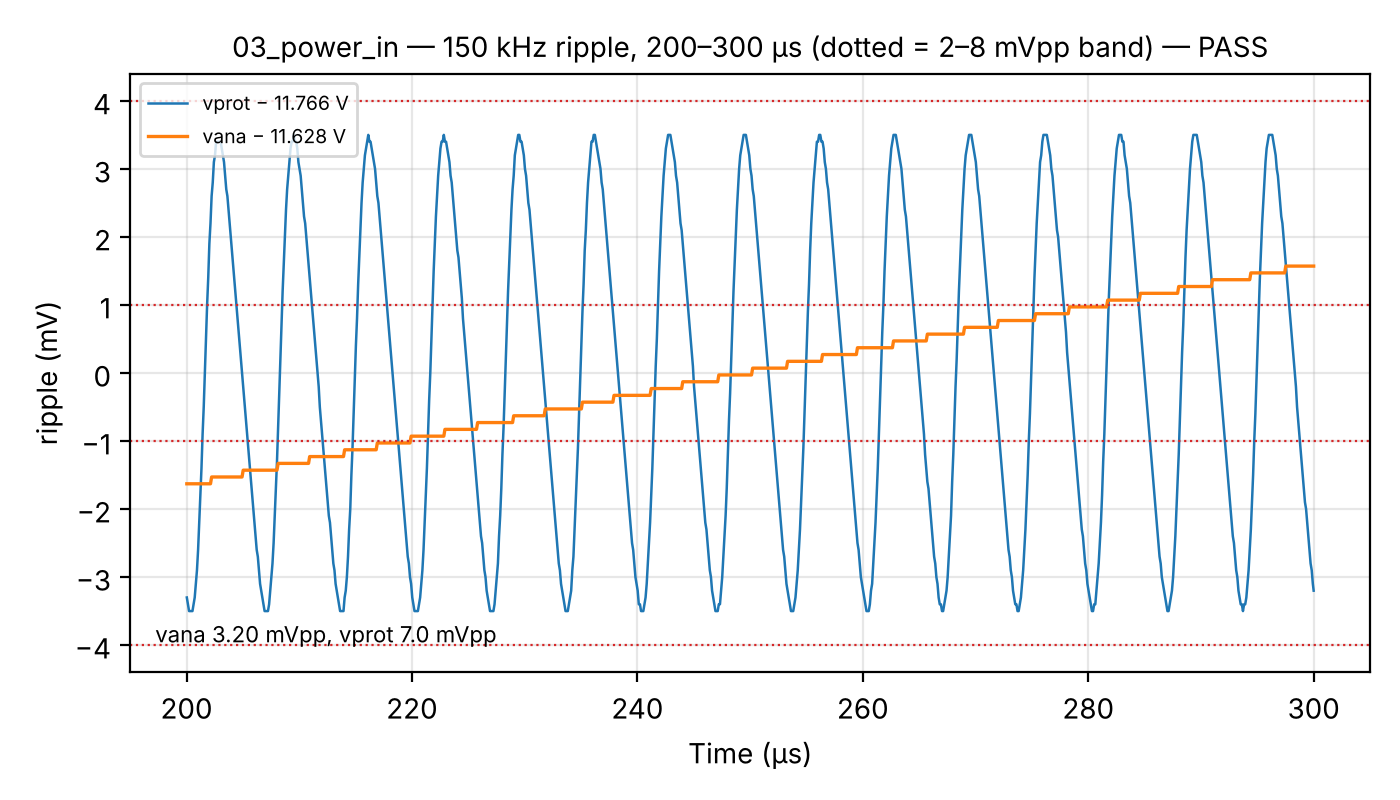
\includegraphics[width=0.85\linewidth,height=0.4\textheight,keepaspectratio]{figures/multisim/03_power_in/03_ripple}\caption{Ripple on the analog rail}\end{figure}
\clearpage
\subsubsection*{Card 4: reverse supply}
\begin{figure}[H]\centering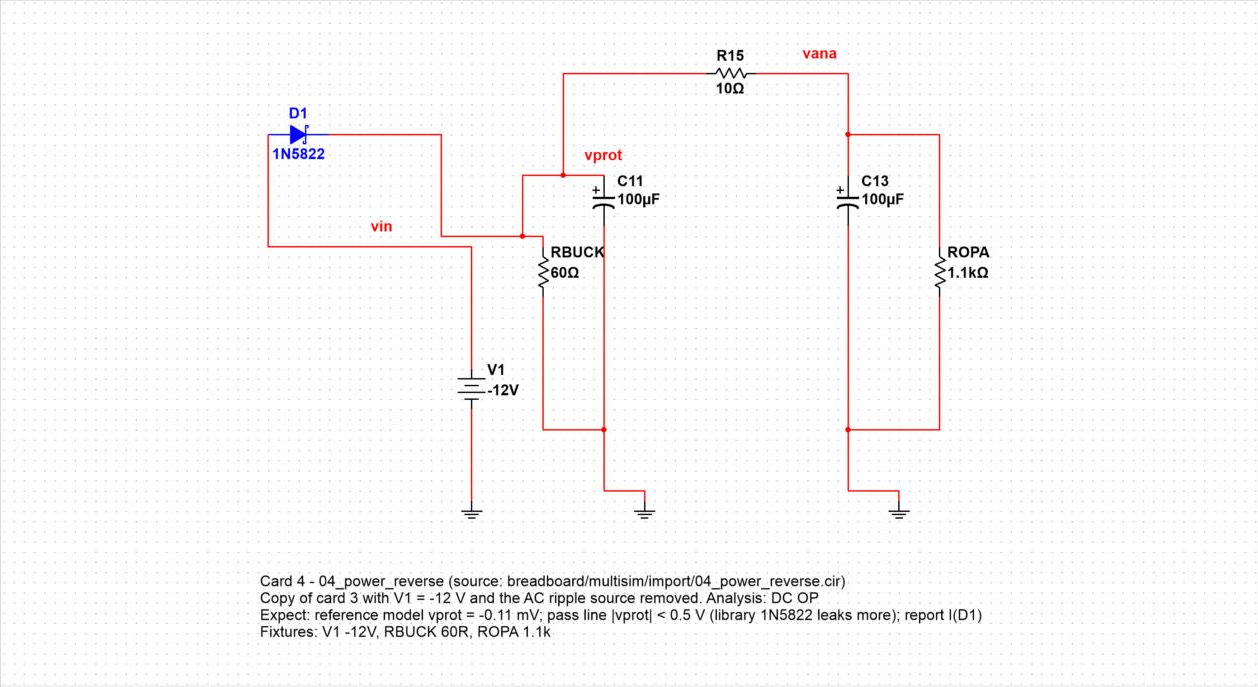
\includegraphics[width=0.85\linewidth,height=0.4\textheight,keepaspectratio]{figures/multisim/04_power_reverse/04_schematic}\caption{Multisim schematic}\end{figure}
\begin{figure}[H]\centering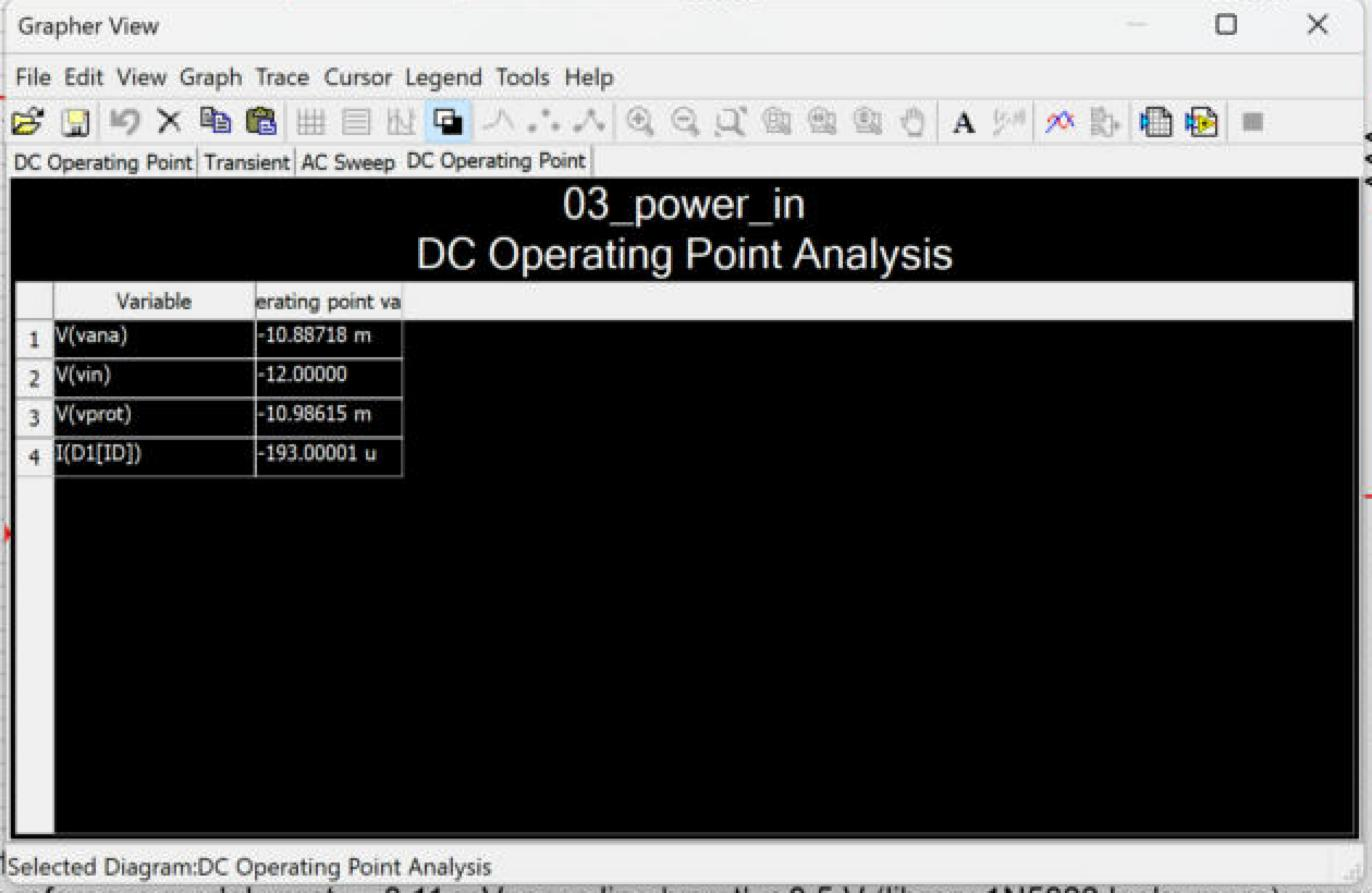
\includegraphics[width=0.85\linewidth,height=0.4\textheight,keepaspectratio]{figures/multisim/04_power_reverse/04_grapher_dcop}\caption{Multisim grapher, DC operating point}\end{figure}
\begin{figure}[H]\centering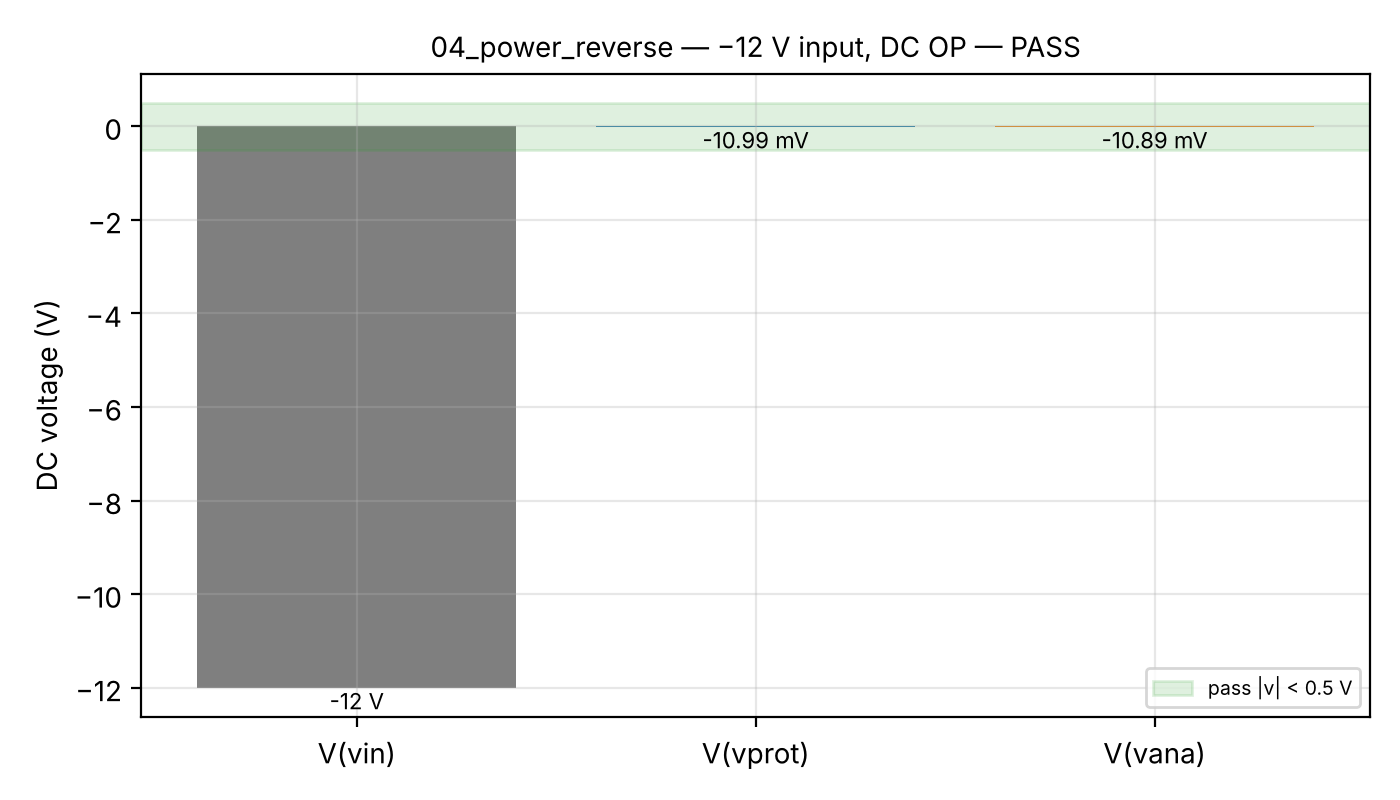
\includegraphics[width=0.85\linewidth,height=0.4\textheight,keepaspectratio]{figures/multisim/04_power_reverse/04_reverse_dc}\caption{Reverse supply DC}\end{figure}
\clearpage
\subsubsection*{Card 5: sync divider}
\begin{figure}[H]\centering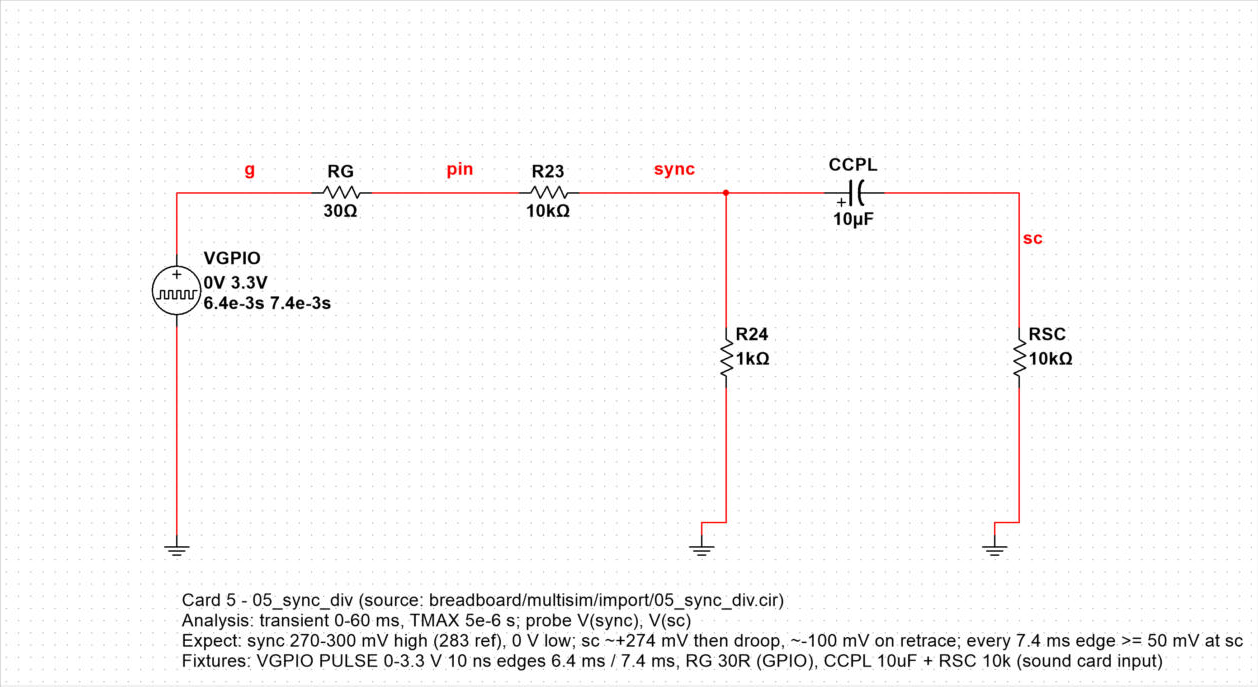
\includegraphics[width=0.85\linewidth,height=0.4\textheight,keepaspectratio]{figures/multisim/05_sync_div/05_schematic}\caption{Multisim schematic}\end{figure}
\begin{figure}[H]\centering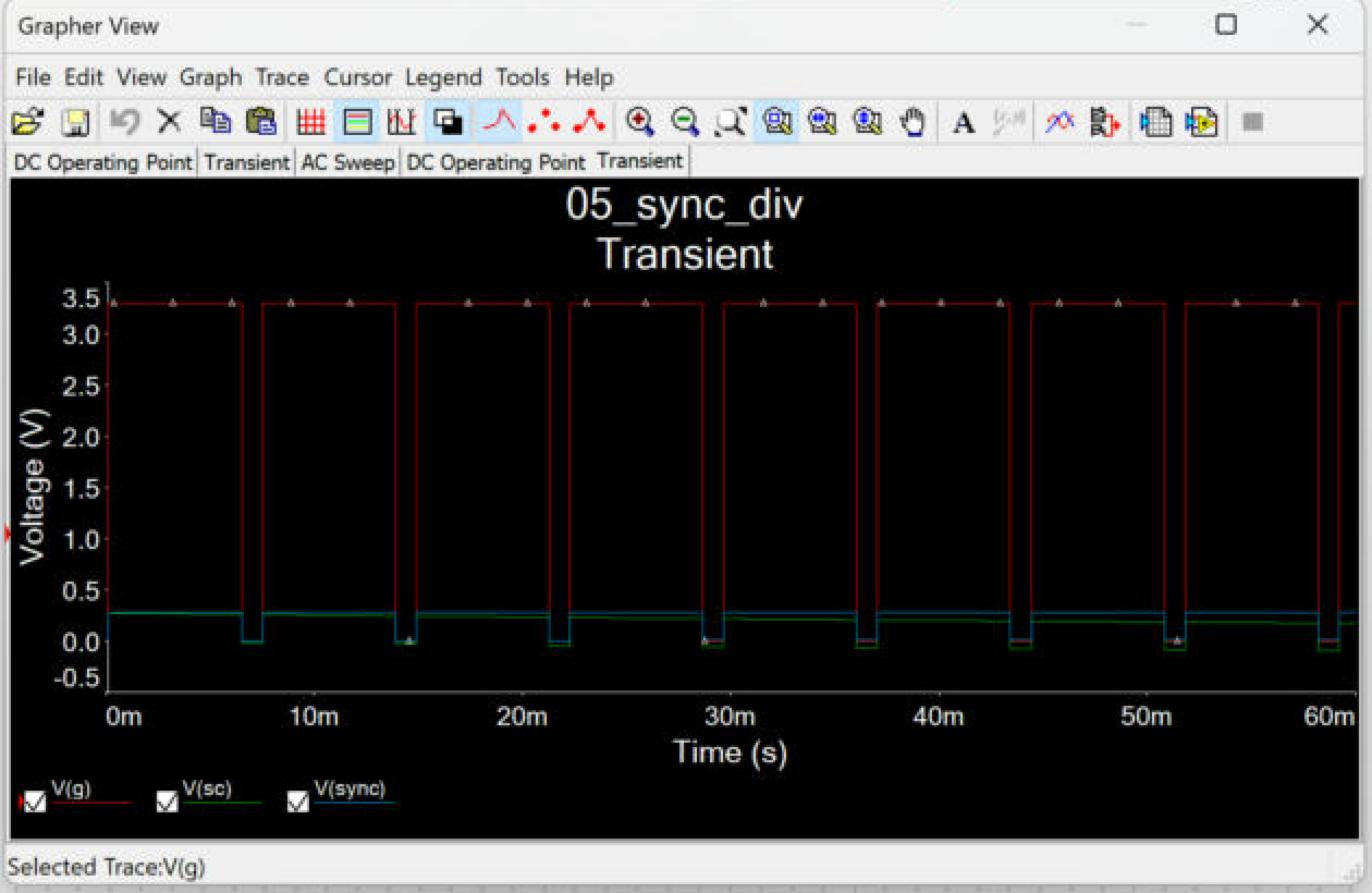
\includegraphics[width=0.85\linewidth,height=0.4\textheight,keepaspectratio]{figures/multisim/05_sync_div/05_grapher_tran}\caption{Multisim grapher, transient}\end{figure}
\begin{figure}[H]\centering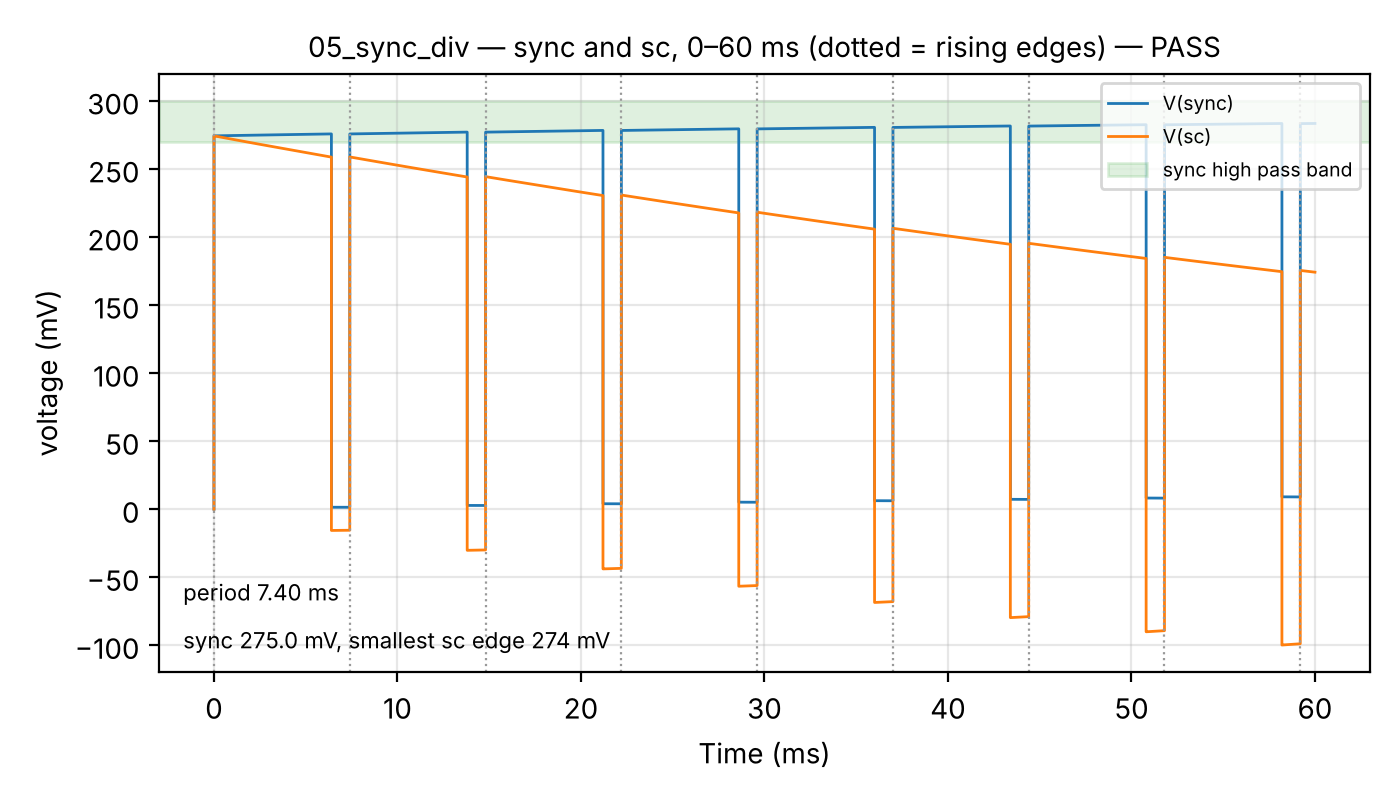
\includegraphics[width=0.85\linewidth,height=0.4\textheight,keepaspectratio]{figures/multisim/05_sync_div/05_sync_sc}\caption{Sync pulse into the sound card}\end{figure}
\clearpage
\subsubsection*{Card 6: IF input}
\begin{figure}[H]\centering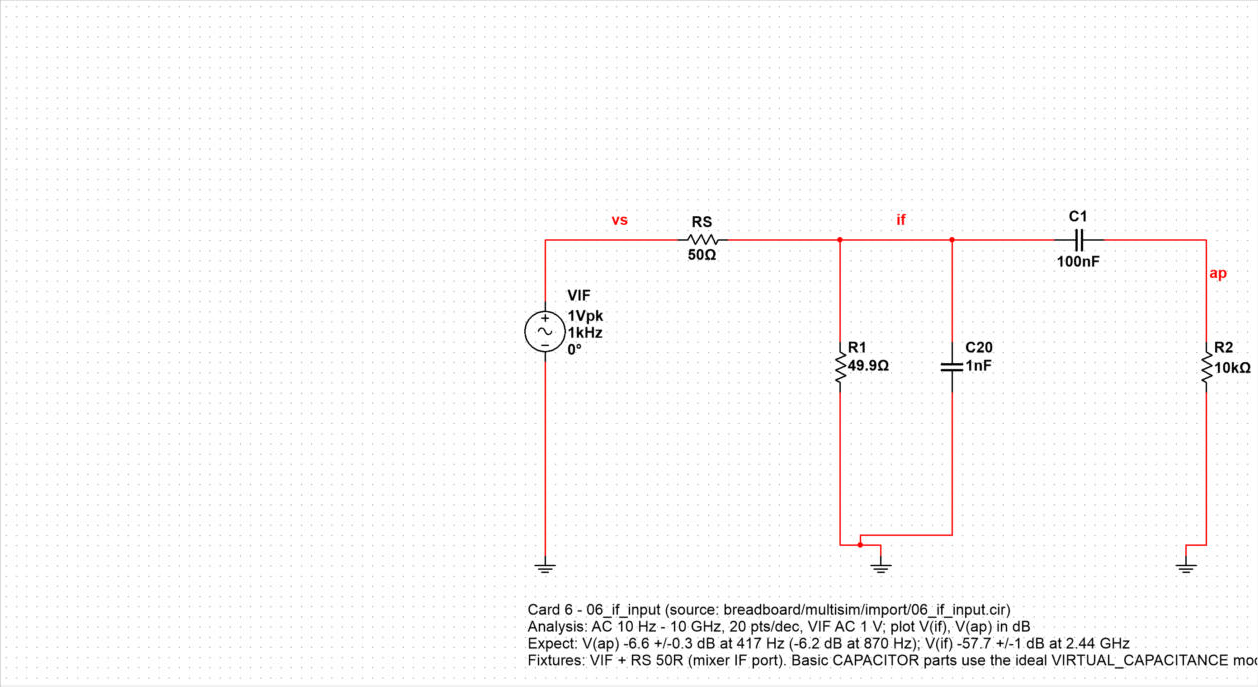
\includegraphics[width=0.85\linewidth,height=0.4\textheight,keepaspectratio]{figures/multisim/06_if_input/06_schematic}\caption{Multisim schematic}\end{figure}
\begin{figure}[H]\centering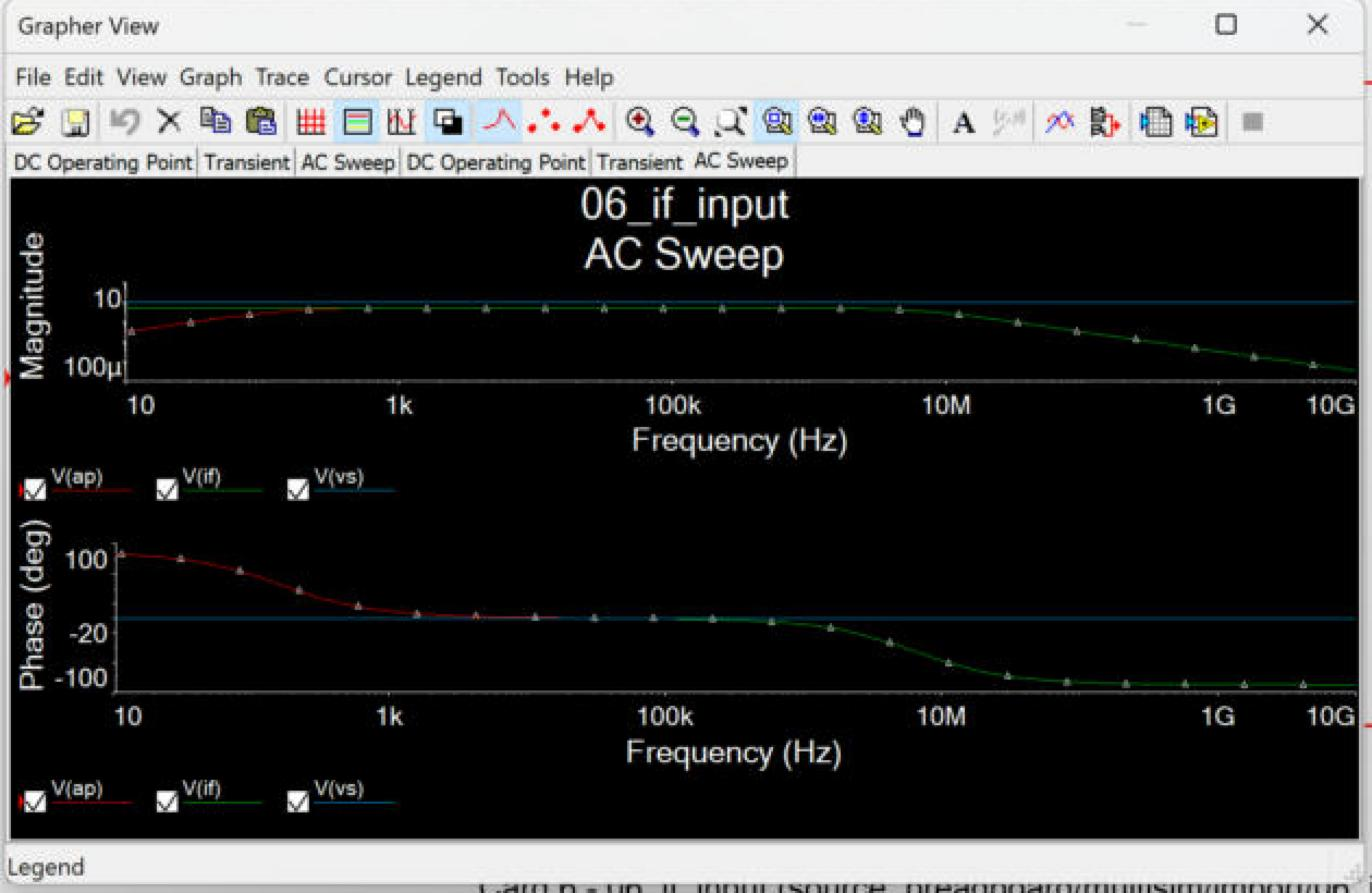
\includegraphics[width=0.85\linewidth,height=0.4\textheight,keepaspectratio]{figures/multisim/06_if_input/06_grapher_ac}\caption{Multisim grapher, AC sweep}\end{figure}
\begin{figure}[H]\centering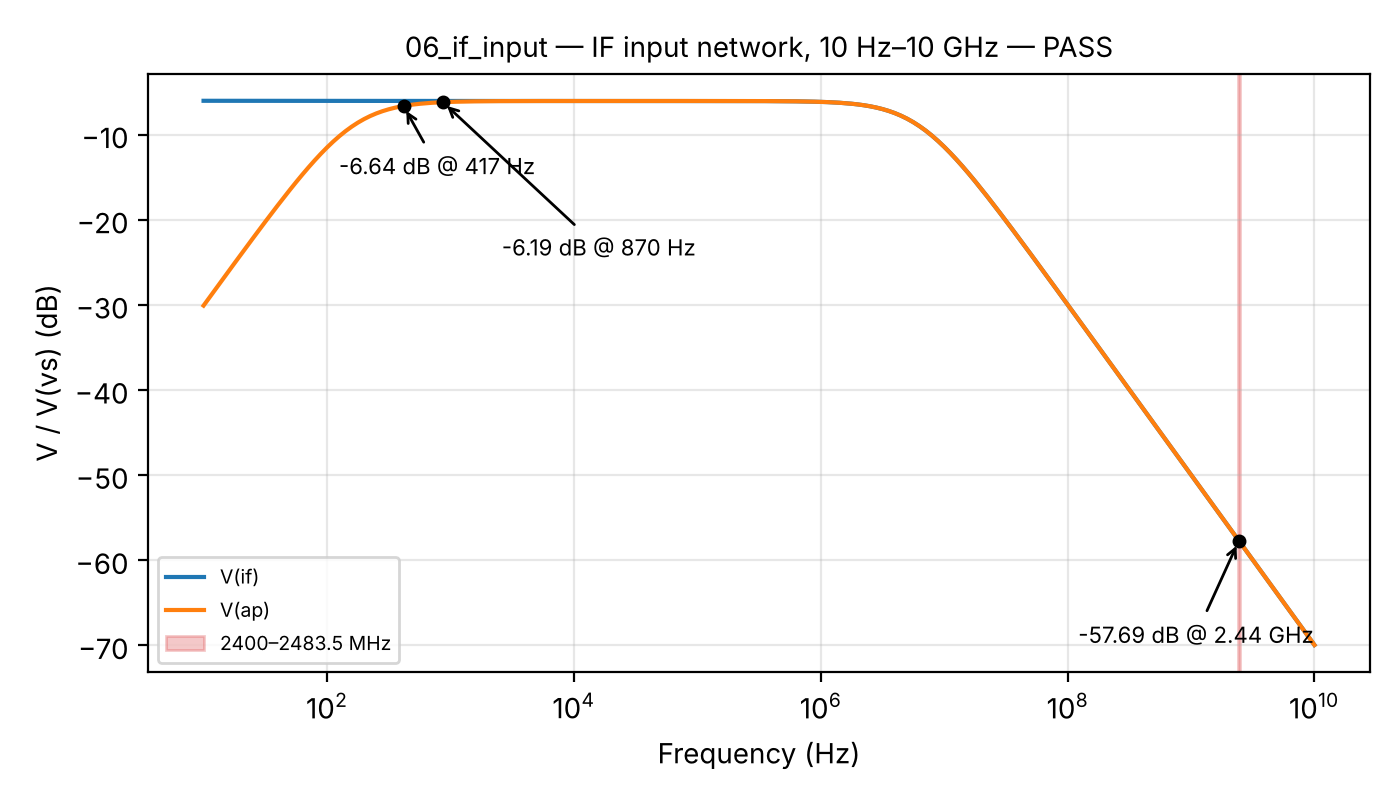
\includegraphics[width=0.85\linewidth,height=0.4\textheight,keepaspectratio]{figures/multisim/06_if_input/06_if_input}\caption{IF input response}\end{figure}
\clearpage
\subsubsection*{Card 7: scaled radar}
\begin{figure}[H]\centering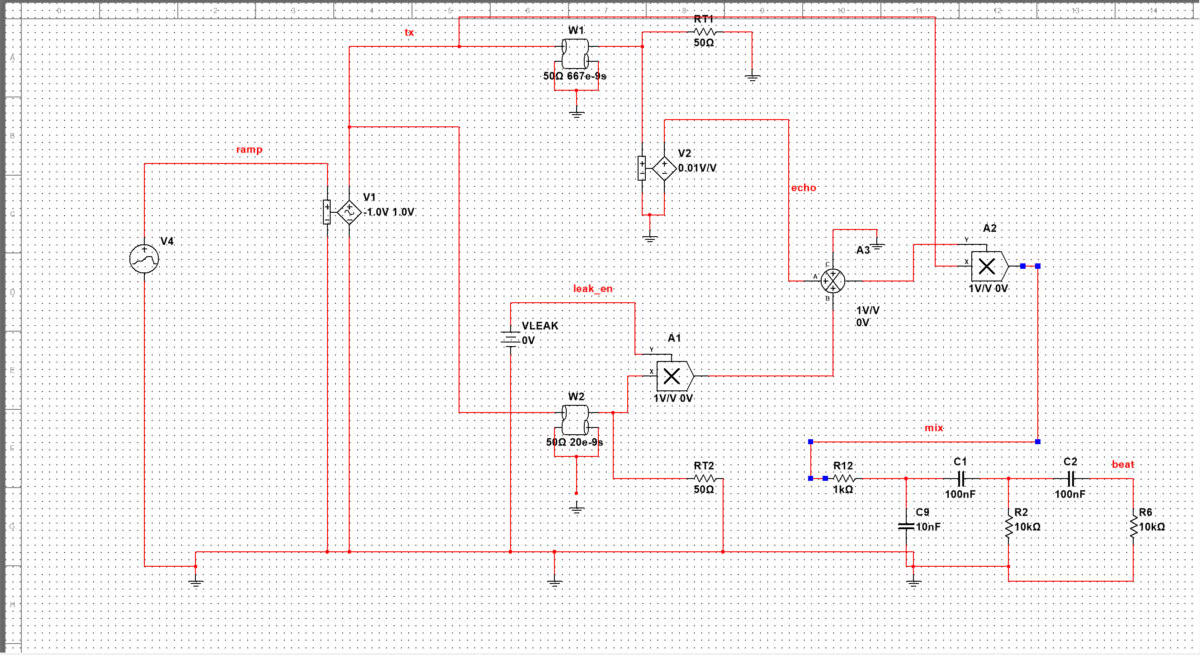
\includegraphics[width=0.85\linewidth,height=0.4\textheight,keepaspectratio]{figures/multisim/07_fmcw_radar/07_schematic}\caption{Multisim schematic}\end{figure}
\begin{figure}[H]\centering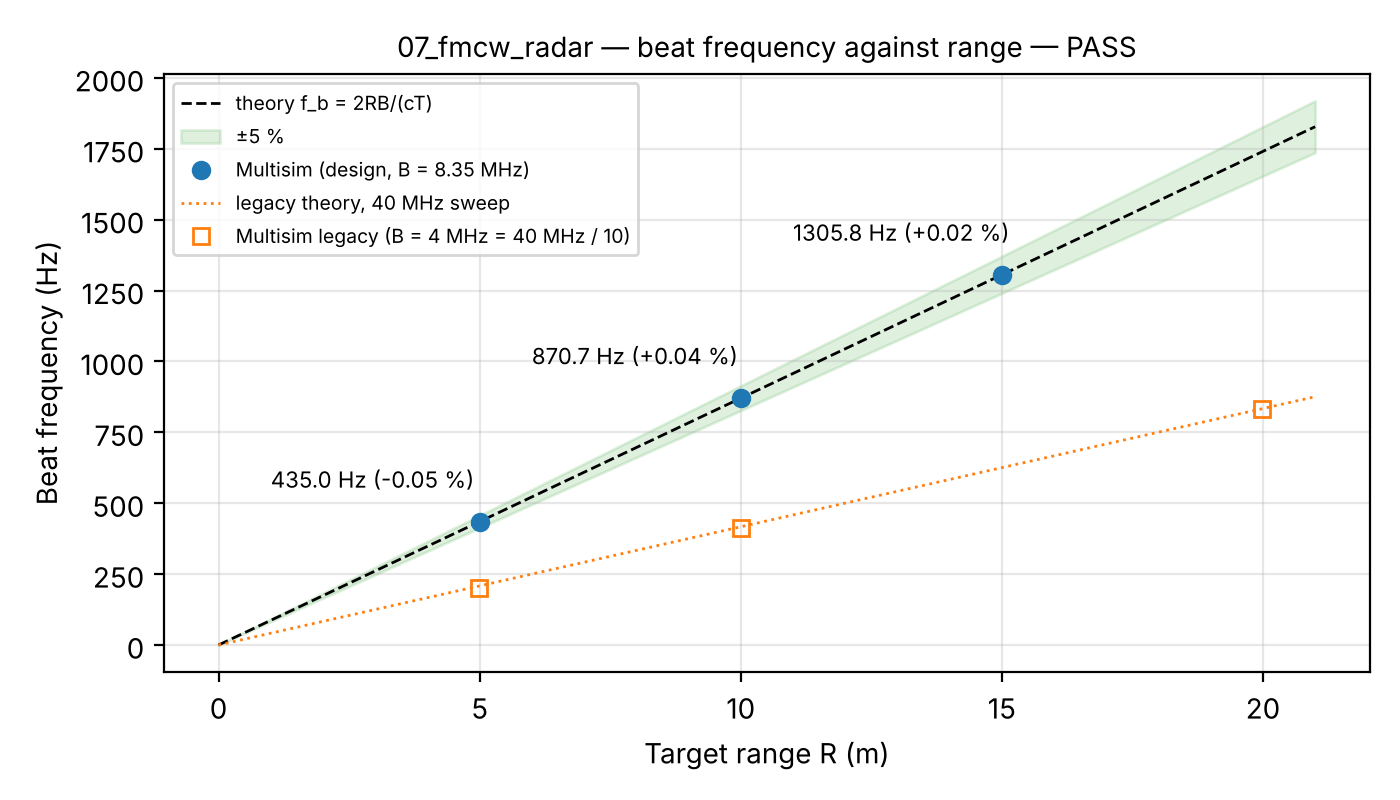
\includegraphics[width=0.85\linewidth,height=0.4\textheight,keepaspectratio]{figures/multisim/07_fmcw_radar/07_beat_vs_range}\caption{Beat frequency vs. range}\end{figure}
\begin{figure}[H]\centering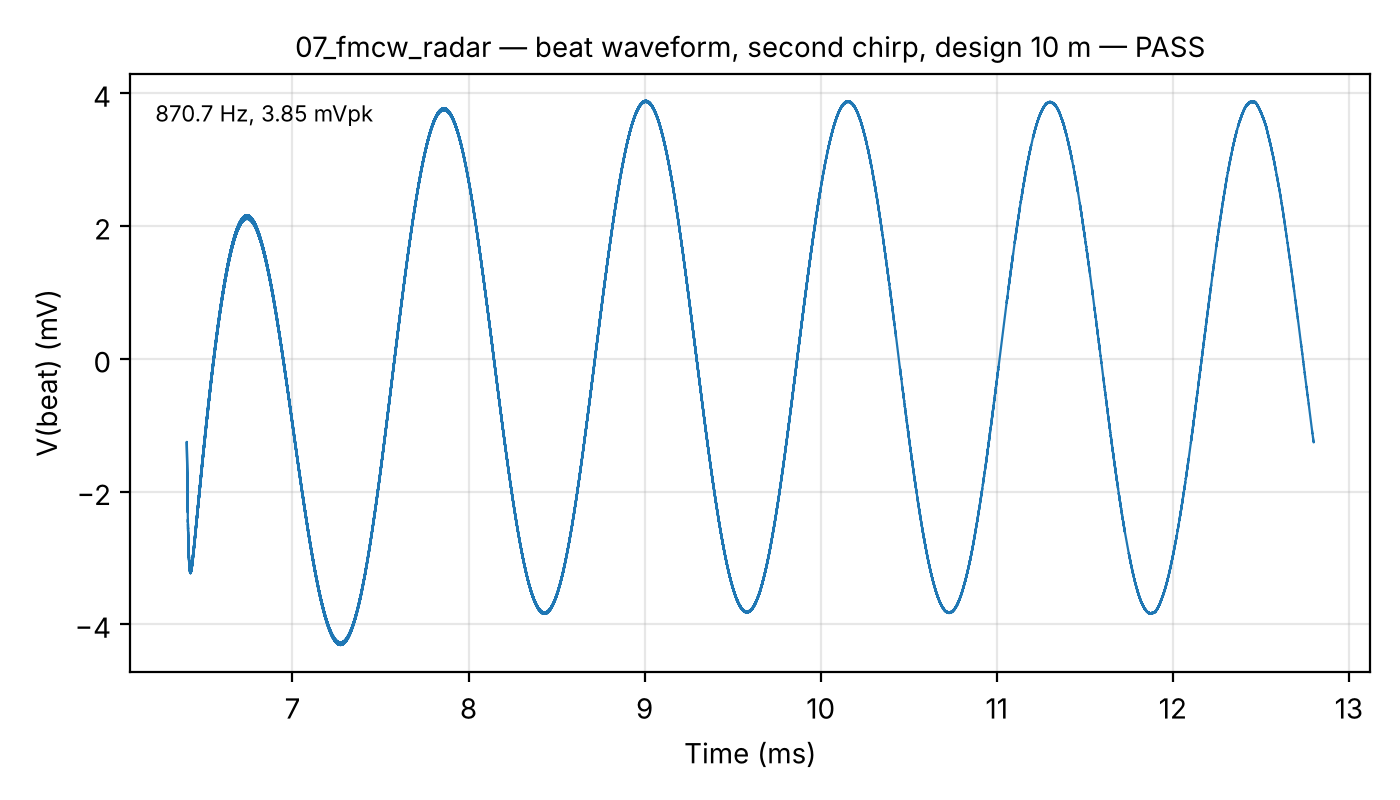
\includegraphics[width=0.85\linewidth,height=0.4\textheight,keepaspectratio]{figures/multisim/07_fmcw_radar/07_beat_waveform}\caption{Beat waveform}\end{figure}
\begin{figure}[H]\centering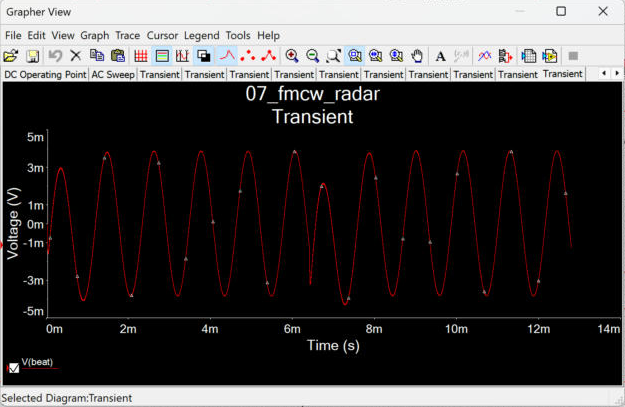
\includegraphics[width=0.85\linewidth,height=0.4\textheight,keepaspectratio]{figures/multisim/07_fmcw_radar/07_grapher_tran_design10m}\caption{Multisim grapher, transient (10 m)}\end{figure}
\begin{figure}[H]\centering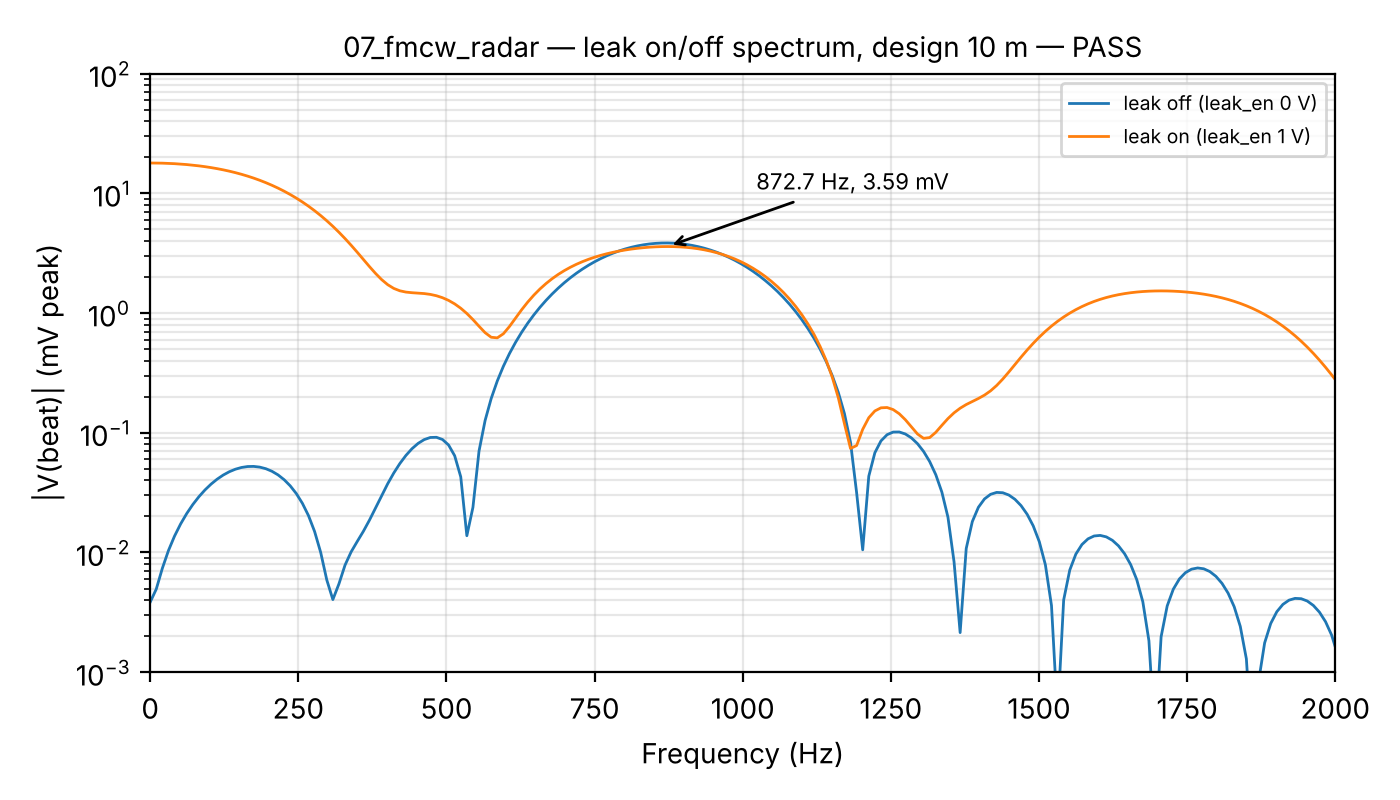
\includegraphics[width=0.85\linewidth,height=0.4\textheight,keepaspectratio]{figures/multisim/07_fmcw_radar/07_leak_on_off}\caption{Spectrum with leakage on/off}\end{figure}
\begin{figure}[H]\centering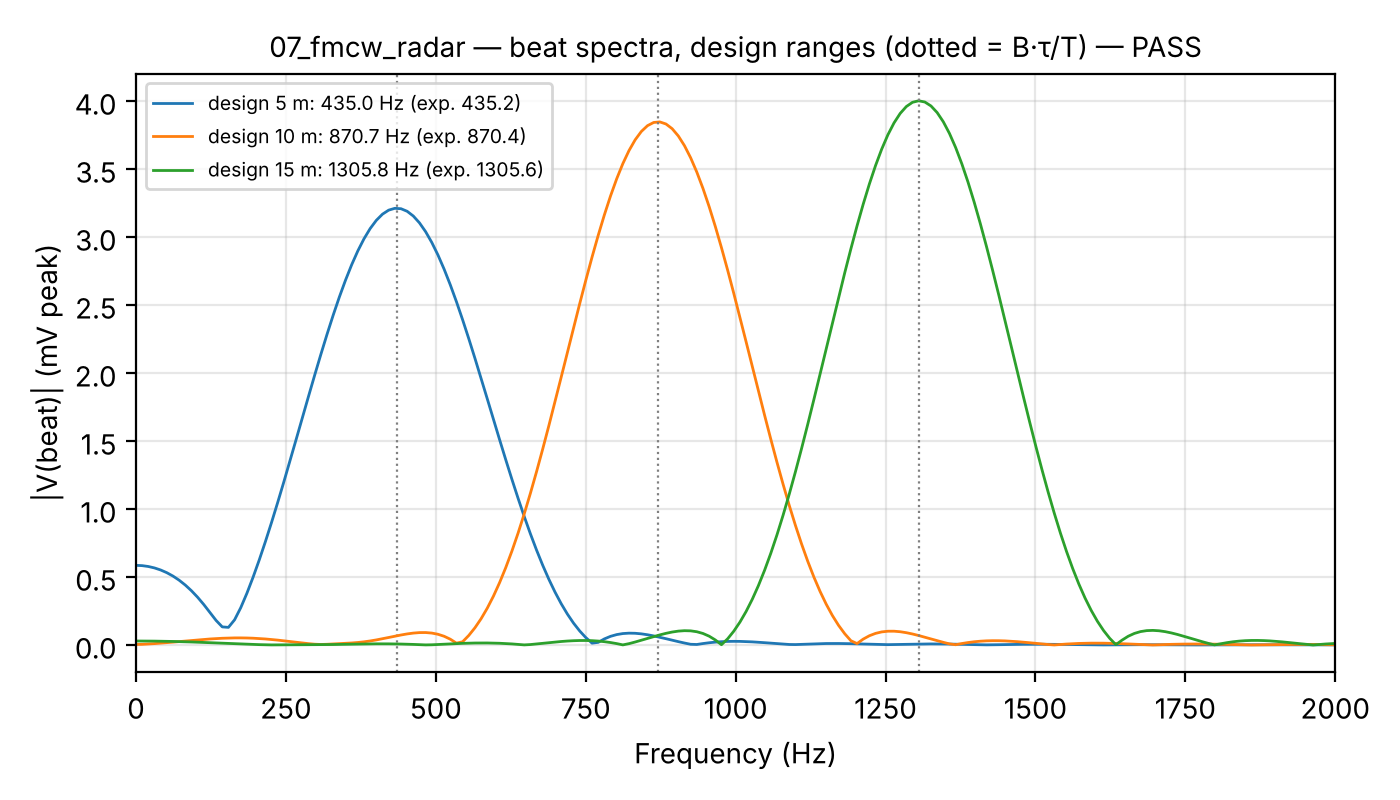
\includegraphics[width=0.85\linewidth,height=0.4\textheight,keepaspectratio]{figures/multisim/07_fmcw_radar/07_spectra_by_range}\caption{Spectra at each range}\end{figure}
\clearpage
\subsubsection*{Card 8: full board}
\begin{figure}[H]\centering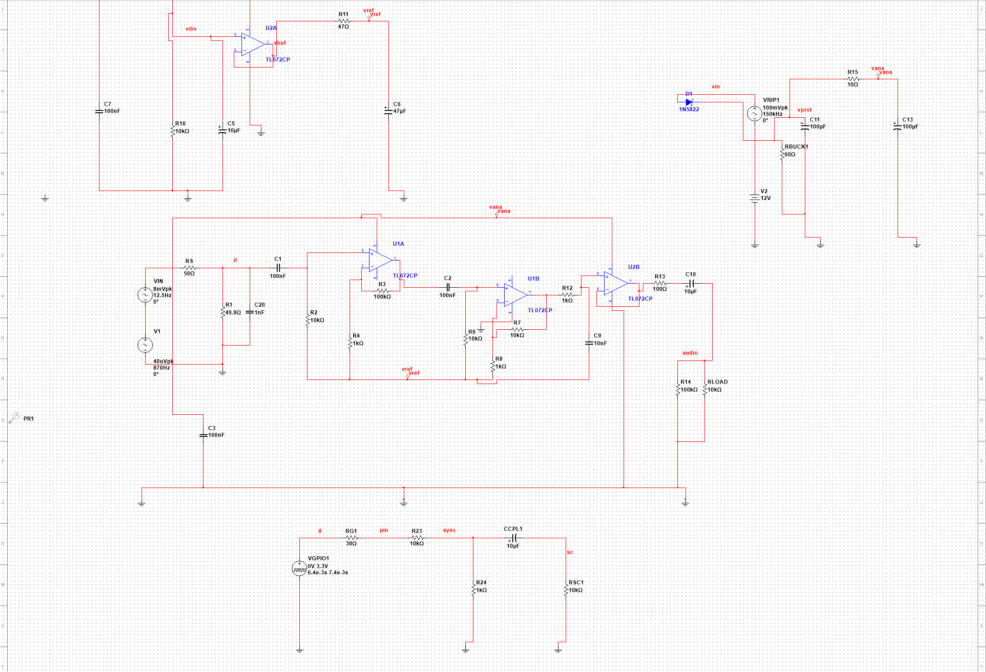
\includegraphics[width=0.85\linewidth,height=0.4\textheight,keepaspectratio]{figures/multisim/08_baseband_system/08_schematic}\caption{Multisim schematic (screenshot from before the supply-pin fix)}\end{figure}
\begin{figure}[H]\centering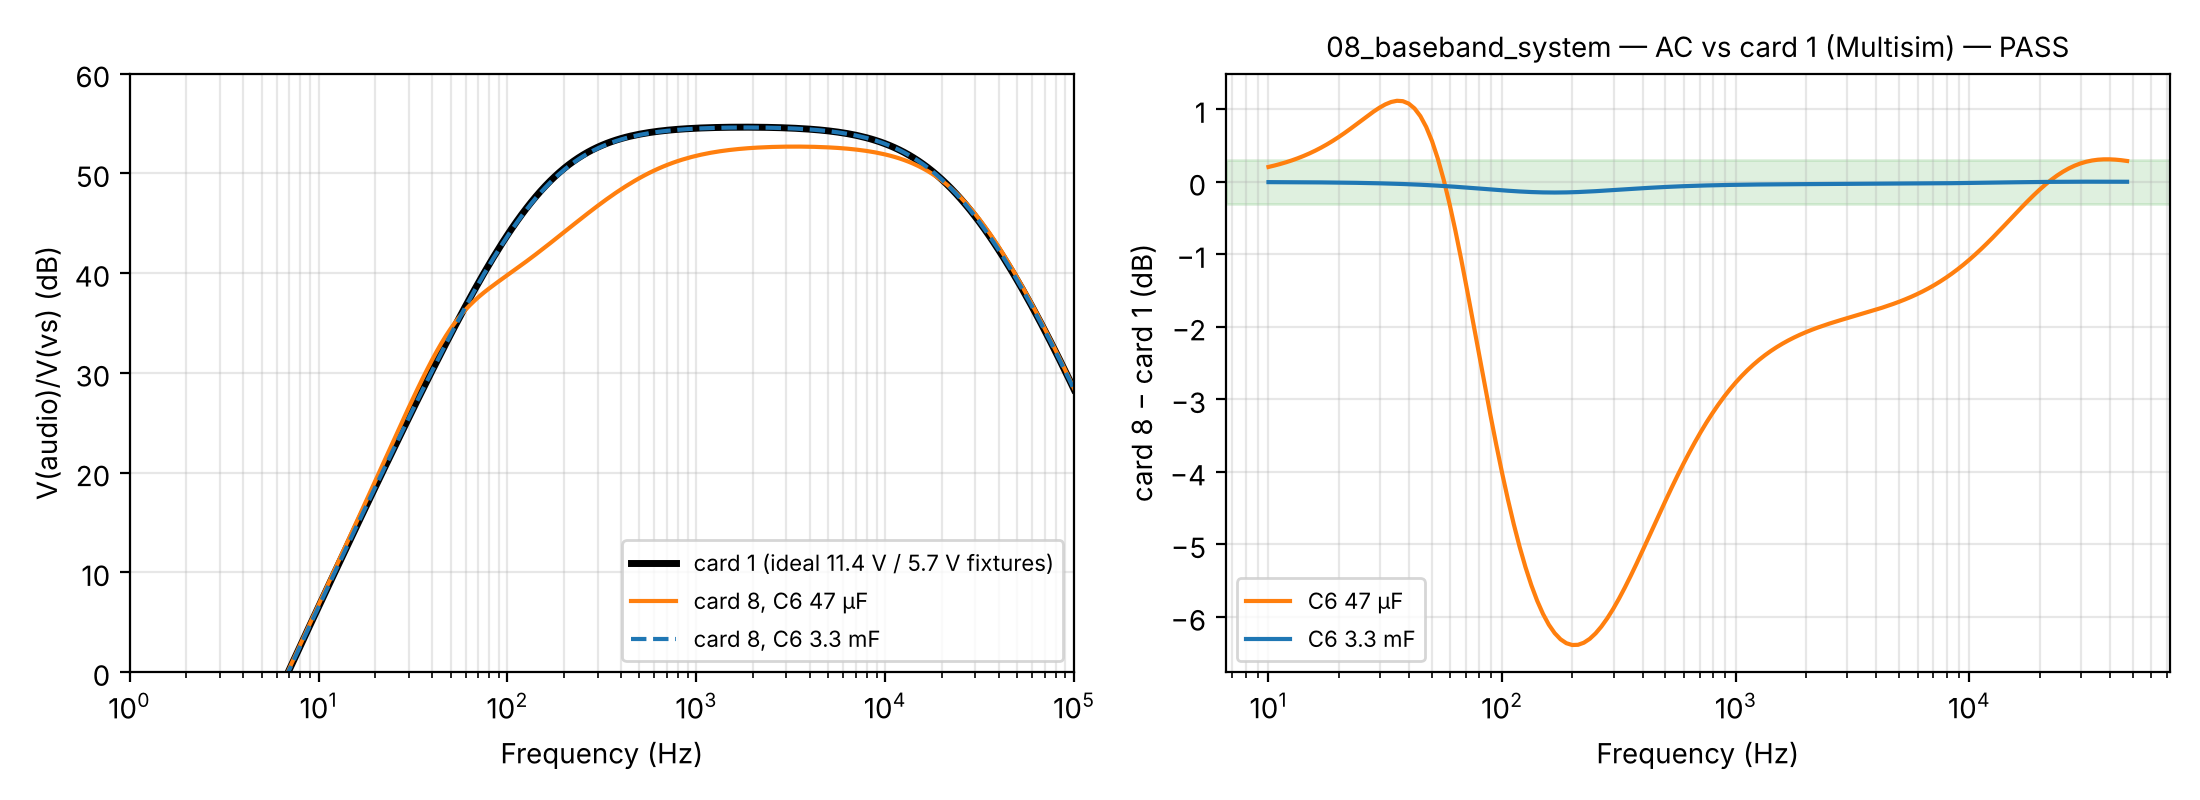
\includegraphics[width=0.85\linewidth,height=0.4\textheight,keepaspectratio]{figures/multisim/08_baseband_system/08_ac_vs_card1}\caption{Gain vs. card 1, C6 47 \textmu F and 3.3 mF}\end{figure}
\begin{figure}[H]\centering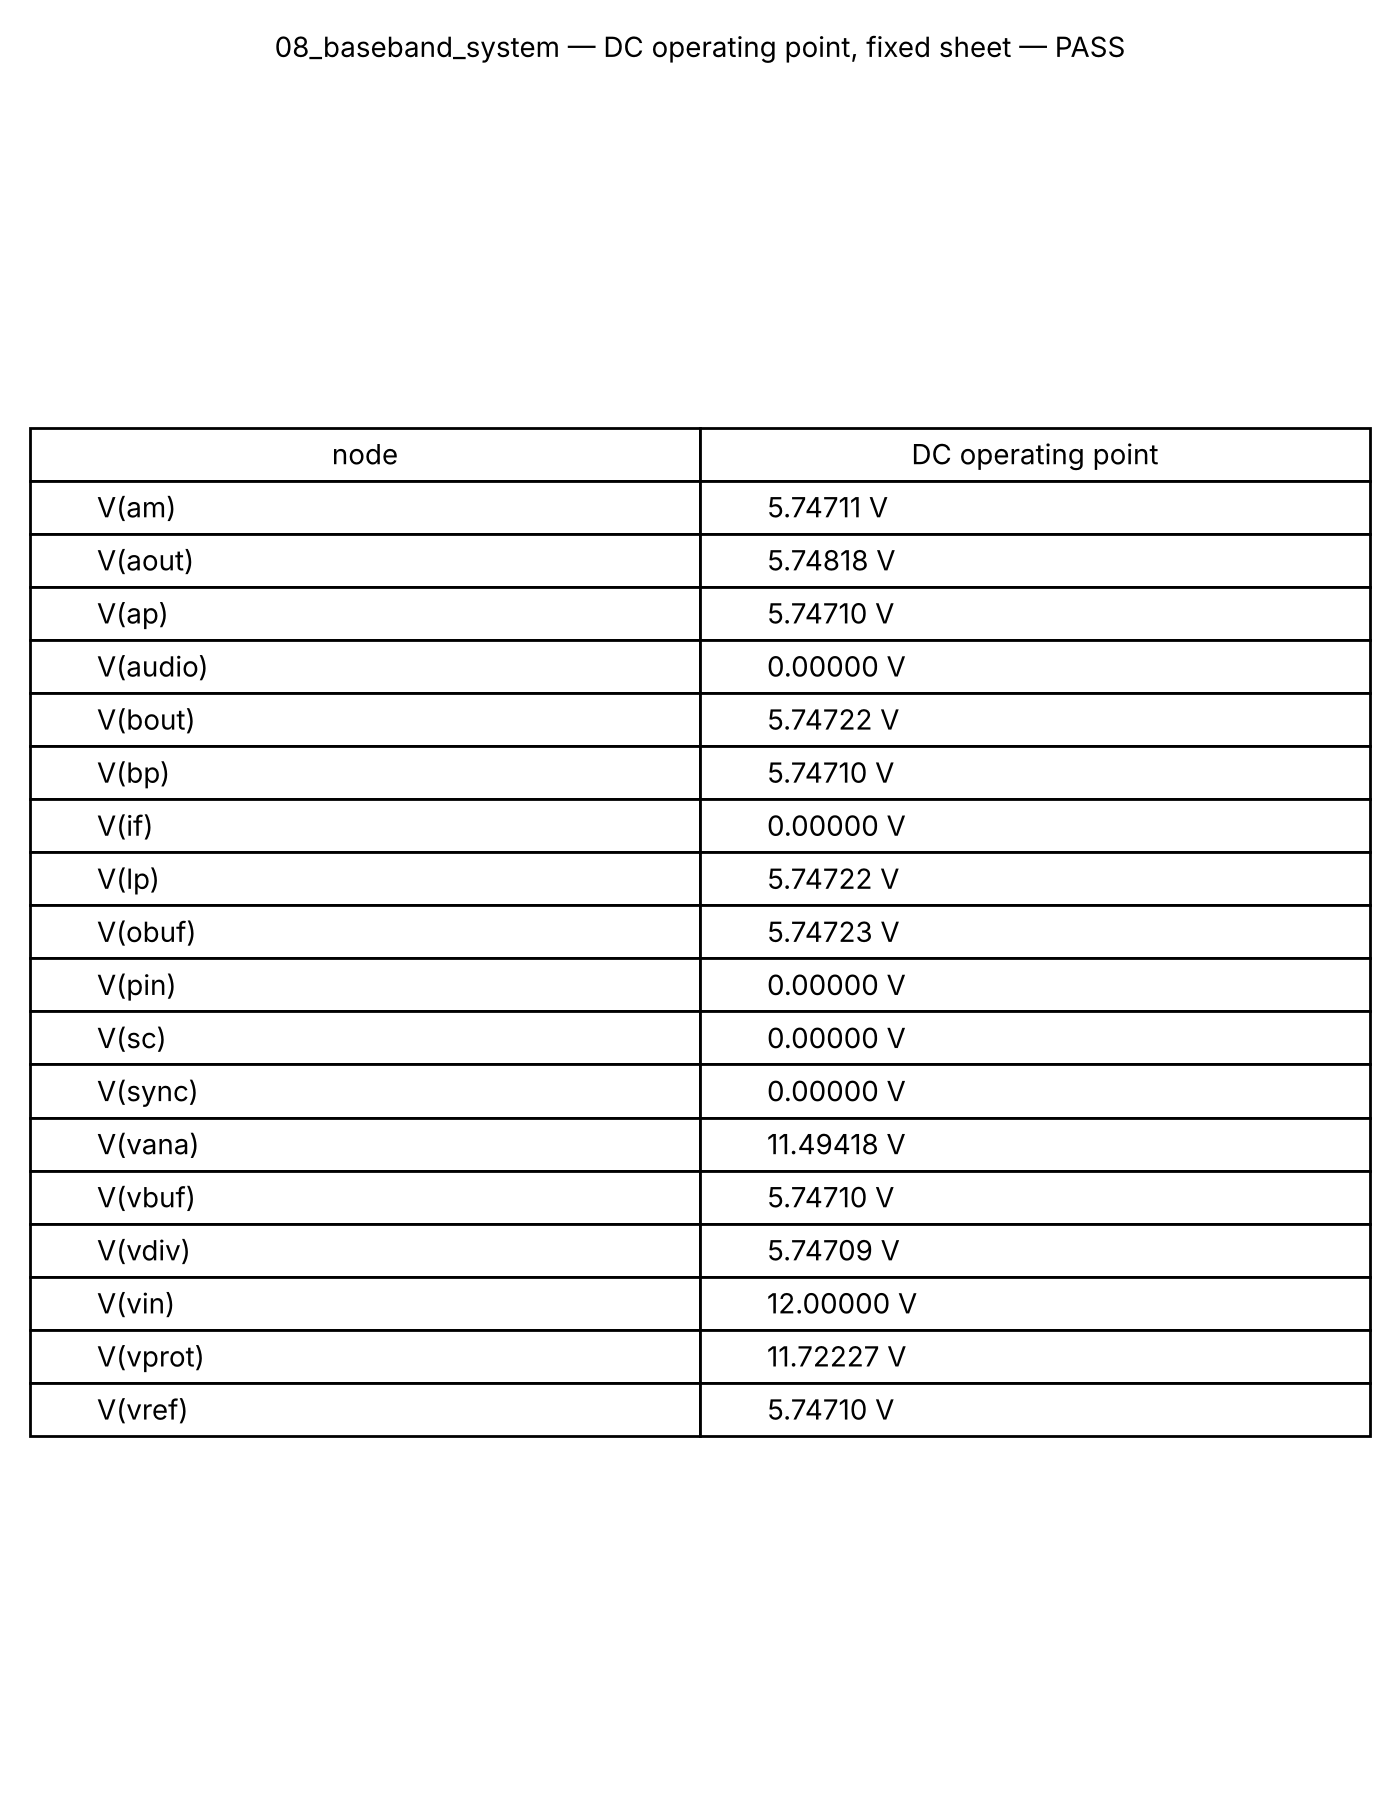
\includegraphics[width=0.85\linewidth,height=0.4\textheight,keepaspectratio]{figures/multisim/08_baseband_system/08_dc_table}\caption{DC operating point, full board (fixed)}\end{figure}
\begin{figure}[H]\centering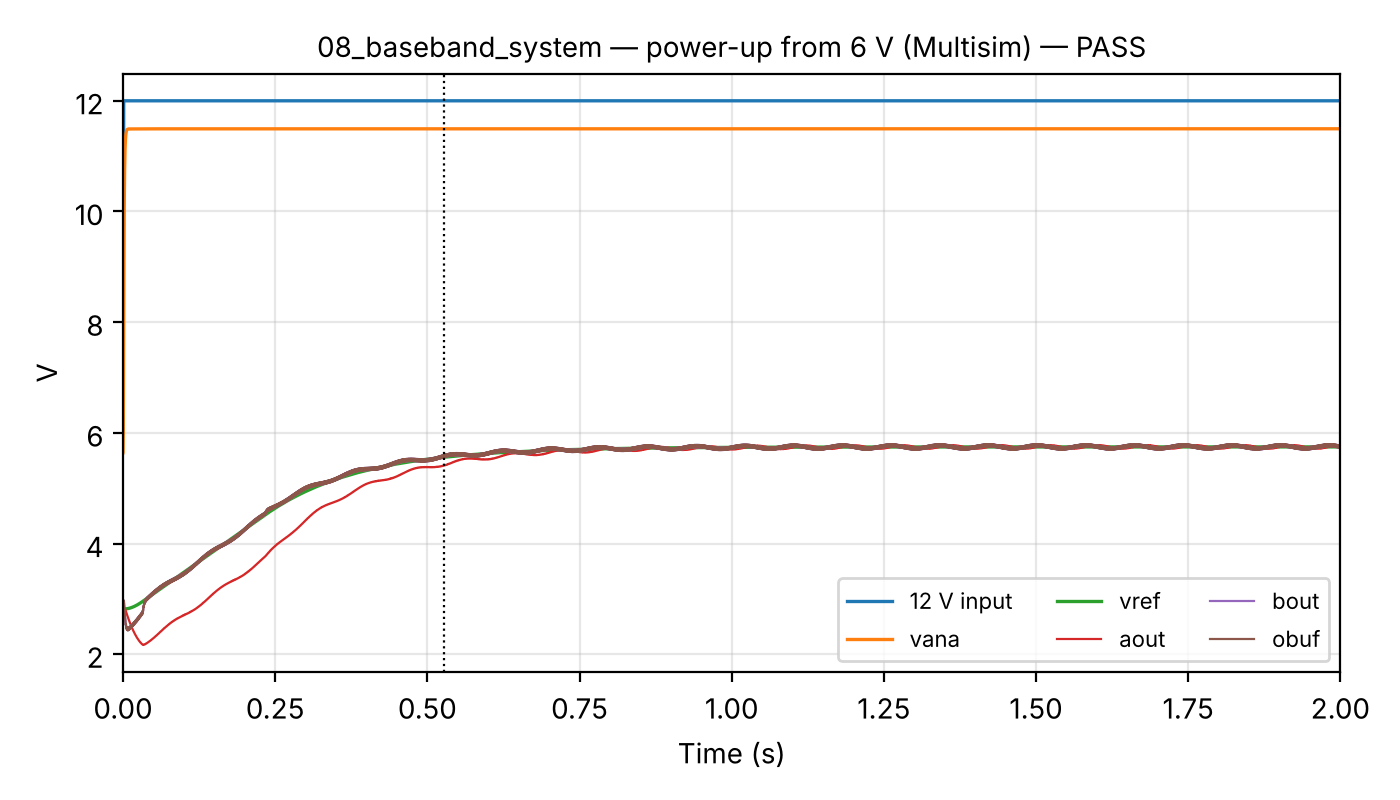
\includegraphics[width=0.85\linewidth,height=0.4\textheight,keepaspectratio]{figures/multisim/08_baseband_system/08_powerup}\caption{Power-up from 6 V}\end{figure}
\begin{figure}[H]\centering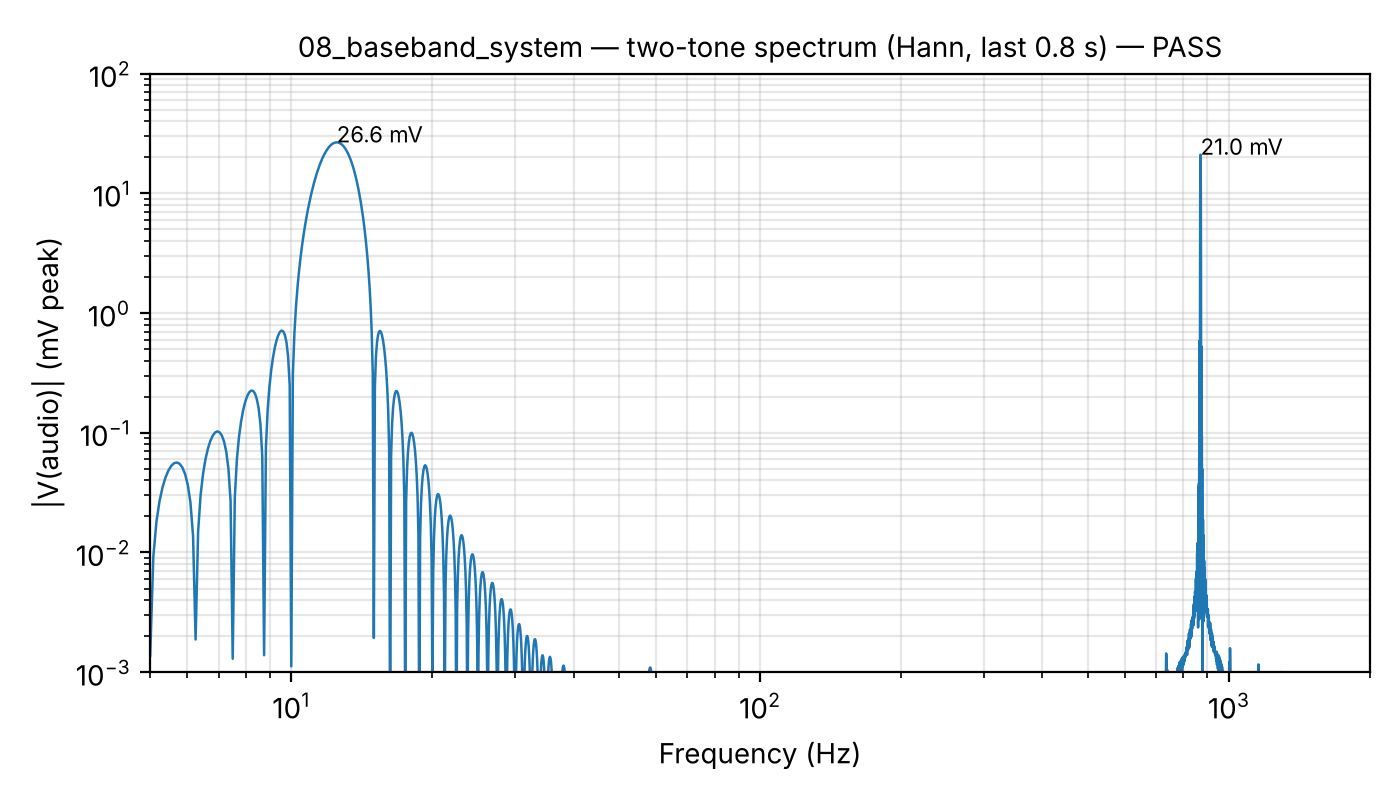
\includegraphics[width=0.85\linewidth,height=0.4\textheight,keepaspectratio]{figures/multisim/08_baseband_system/08_twotone_spectrum}\caption{Two-tone spectrum, full board}\end{figure}
\clearpage
\end{document}
